\documentclass[a4paper,11pt]{article}
\pdfoutput=1 % if your are submitting a pdflatex (i.e. if you have
         % images in pdf, png or jpg format)

\usepackage{jcappub} % for details on the use of the package, please
                 % see the JCAP-author-manual

\usepackage{hyperref}
\usepackage{amsmath}

\usepackage[english,activeacute]{babel} 
\usepackage[toc,page]{appendix}
\usepackage{graphicx}
\usepackage{color}
\usepackage{tensor}

\usepackage{xcolor}
\usepackage{graphicx}
\usepackage{colortbl}
\usepackage{placeins}
\usepackage[margin=2.5cm]{geometry}
\usepackage{multirow}

\usepackage[utf8]{inputenc}

% command for co-polarized
\newcommand{\co}{\mathbin{\|}}

% command for cross-polarized
\newcommand{\cx}{\mathbin{\times}}


\title{\boldmath Pixel space convolution for cosmic microwave background experiments}


%% %simple case: 2 authors, same institution
%% \author{A. Uthor}
%% \author{and A. Nother Author}
%% \affiliation{Institution,\\Address, Country}

% more complex case: 4 authors, 3 institutions, 2 footnotes
\author[a]{P. Flux\'a, }
\author[b]{M.K. Brewer, }
\author[a]{R. D\"unner.}

% The "\note" macro will give a warning: "Ignoring empty anchor..."
% you can safely ignore it.

\affiliation[a]{Instituto de Astrof\'isica, Pontificia Universidad Cat\'olica de Chile ,\\Vicu\~na Mackenna 4860, Chile}
\affiliation[b]{Department of Astronomy, Johns Hopkins University,\\Baltimore MD, USA}

% e-mail addresses: one for each author, in the same order as the authors
\emailAdd{pedro@fluxanet.net}
\emailAdd{mkb email goes here}
\emailAdd{rdunner@astro.puc.cl}



\abstract{
	Cosmic microwave background experiments have experienced an exponential increase in complexity, data size and sensitivity. Current and future experiments aim at characterizing the B-mode power spectrum which, due to its faintness, will require extreme control over systematic effects. One of such effects might arise by the complex coupling between the telescope beam and its scanning strategy. In this work, we present a new software tool, the Pixel Space COnvolver, PISCO, capable of producing mock data streams for a general CMB experiment. We show results of an application of PISCO to the Cosmology Large Angular Scale Surveryor, and its Q-band telescope. Results show that beam eccentricity might cause a temperature to polarization leakage above $\ell \approx 50$. }

\begin{document}
\maketitle
\flushbottom

% enable numbering of equations that considers the section number
%\numberwithin{equation}{section}

\section{Introduction}

% gives the width of the current document in pts
\showthe\textwidth

The study of the cosmic microwave background (CMB) in the last few decades has lead to major advances in Cosmology. In particular, the study of the temperature and polarization anisotropy field has allowed us to achieve percent level constraints on cosmological parameters, favoring a universe dominated by cold dark matter plus a cosmological constant ($\Lambda$CDM), known today as the standard model of Cosmology {\color{red} (cite most relevant papers including WMAP and Planck)}. Current efforts are mostly focused on the polarization anisotropy field, as it promises to provide independent constraints on the very early stages of the Universe. At these very first moments, the leading theory claims that the Universe exponentially expanded nearly 60 e-folds in a process called Inflation, becoming the flat, homogeneous and isotropic Universe that we see today. If true, gravitational waves generated by this expansion would have later interacted with the surface of last scatter, leaving a unique imprint in the polarization field which should be observable today.

CMB anisotropies form a Gaussian field on the sky, being nearly 10\% polarized. The latter can be modeled as a spin-2 field, which is separable in two orthogonal components: a curl-free component called E-mode, and a divergence-free component called B-mode. In the absence of gravitational waves, the polarization field would contain only E-modes, which would be partially turned into B-modes by gravitational waves acting during the epochs of recombination and reionization. The resulting B-mode field would be one or two orders of magnitude lower than the E-mode signal, being very faint and difficult to measure. Moreover, recent results show that this signal lies below other foreground signals like gravitational lensing distortions induced by the matter distribution and polarized emissions from the interstellar medium {\color{red}(add cites)}. Thus, detecting the primordial B-mode signal has become a major technical challenge.

Another source of confusion are experimental systematic effects. The tremendous increase in sensitivity of CMB experiments have brought into stage a long list of instrumental and observational effects, which need to be properly incorporated into the data reduction process, as well as for the design of future experiments. Being this an extended signal on the sky, understanding effects the detailed polarized antenna response of the telescope, and how it gets convolved with the sky signal (scan strategy), is key, as it can directly affect the scientific results.

The main beam is where most of the radiation is captured by the antenna, and thus the effects of the beam shape and polarization have been extensively studied. 
%Analytic techniques
It has been shown that symmetrical beams with smooth profiles can be analytically accounted for when computing the power spectra of CMB maps (see \cite{2003ApJS..148...39P}).
However, beam and pointing mismatch can produce leakage between temperature and polarization (T to P), or between E-modes and B-modes (P to P). The impact of these effects on the maps, power spectra and scientific results, together with mitigation techniques, have been proposed by \cite{PhysRevD.77.083003, 2007MNRAS.376.1767O, 2015JCAP...03..048D}.

The problem becomes much more complicated when sidelobes are included, forcing the use of numerical methods to understand their effects.
Several of these techniques rely on harmonic space representations of the beam, the sky and the scan strategy (\cite{2001PhRvD..63l3002W,2000PhRvD..62l3002C}). Harmonic space algorithms can also exploit redundancies in the computation that allow Fast Fourier Transform (FFT) techniques to be used. An excellent description of FFT-based algorithms, as well an implementation and application to a realistic CMB experiment is given in \cite{2018arXiv180905034D}. On the other hand, pixel space algorithms can account for time-varying effects, like transient events on the sky model, modulation techniques and optical distortions. The work of \cite{2011ApJS..193....5M} describes such an implementation, and its application to the Planck satellite mission.

%Planks approach ... 
The Planck experiment developed Full Focal Plane (FFP) simulations (see \cite{2016A&A...594A..12P}). At the time they were performed, FFP simulations took more than four million CPU-hours on a world-class supercomputer, and required almost 18 TB of storage. FFP simulations included very detailed noise models of the Planck mission and helped, among other things, to provide excellent constraints on the the cosmological parameters and their associated statistical errors (see \cite{2016A&A...594A..13P}). FFP simulations showed that effort on improving tools aiming at simulating CMB experiments will become valuable for current and future missions.

%O'dea approach ...



In this work, we describe the algorithm and prototype implementation of a new CMB computer simulation code, the Pixel Space COnvolver (PISCO). PISCO has the capability of accounting for arbitrary shaped, time-varying beams and sky models. Full polarization treatment of the beam properties is based on the work presented in \cite{2007MNRAS.376.1767O}. PISCO also exploits the massively parallel architecture of Graphics Processing Units (GPU), via the CUDA platform, and was designed from scratch to take advantage of HPC environments.

This paper is organized as follows. 
\S\ref{sec::coordinate-systems} contains a description of the coordinate system and geometrical transformations used to model an antenna pointing at the sky.
\S\ref{sec::antennas} presents a brief introduction to antenna theory. 
\S\ref{sec::pixel_conv} describes the algorithm used by PISCO, as well as a prototype implementation. 
\S\ref{sec::validation} presents validation tests to assess the performance of PISCO. 
\S\ref{sec::class_pisco_sim} provides an example application of PISCO to CLASS (\cite{2016SPIE.9914E..1KH}). 
The paper concludes with a brief discussion on the results obtained in \S\ref{sec::conclusions}.

%
\section{Coordinates}
\label{sec::coordinate-systems}

\subsection{Definitions}

\begin{figure*}
	\centering
	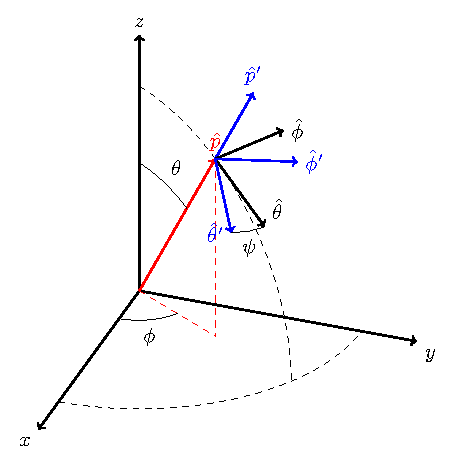
\includegraphics[width=0.47\linewidth]{tikz/sky_basis}	
	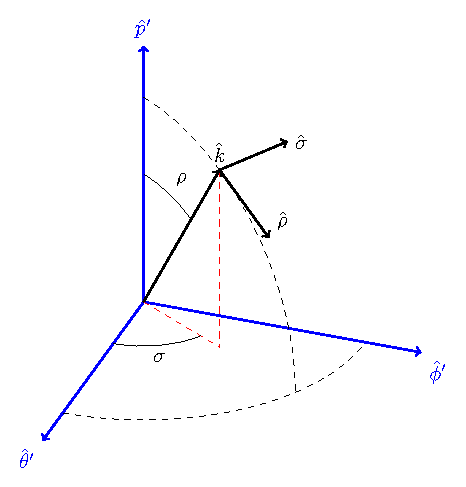
\includegraphics[width=0.47\linewidth]{tikz/beam_basis}
	\caption{Left panel: sky basis. The sky basis is a generic spherical coordinate system. $\hat{x}$, $\hat{y}$ and $\hat{z}$ form an orthonormal basis. Unit vector $\hat{p}$ is defined by its spherical coordinates, co-latitude $\theta$ and longitude $\phi$. Co-latitude increases from the north pole towards the south pole. Longitude increases from west to east. Tangent vectors at $\hat{p}$, $\hat{\theta}$ and $\hat{\phi}$, can be rotated around $\hat{p}$ by angle $\psi$ to generate vectors $\hat{\theta}'$ and $\hat{\phi}'$. Note an observer looking towards the sky along $\hat{p}$ will measure angle $\psi$ as increasing clockwise from South. Right panel: antenna basis. The antenna basis is another orthonormal basis, very much like the sky basis. A unit vector $\hat{k}$ is described by $\rho$ (co-latitude) and $\sigma$ (longitude). Tangent vectors at $\hat{k}$ are $\hat{\rho}$ and $\hat{\sigma}$. }
	\label{fig::sky_basis} 
\end{figure*}

Since PISCO performs the convolution of the polarized antenna response with the sky in ``real'' domain, it makes extensive use of coordinate transformations. These operations can be described by the use of two complementary spherical coordinate systems, which are described in figure \ref{fig::sky_basis}. The first coordinate system corresponds to the \textsl{sky basis}. Unit base vectors of these coordinate system are $\hat{x}$, $\hat{y}$ and $\hat{z}$. For convenience, the antenna pointing in the sky basis will be described as a 3-tuple $\bar{q}$, so that an antenna aiming at co-latitude $\theta_0$ and longitude $\phi_0$, with position angle $\psi_0$ has a pointing 

\begin{equation}
\begin{aligned}
\bar{q}_0= (\theta_0,\phi_0,\psi_0)
\end{aligned}
\end{equation}

Then the \textsl{pointing direction}, denoted by vector $\hat{p}_0$, can be expressed as a linear combination of base vectors and spherical coordinates $(\theta_0,\phi_0)$ via

\begin{equation}
\begin{aligned}
\hat{p}_0 = \cos(\phi_0)\sin(\theta_0)\hat{x} + \sin(\phi_0)\sin(\theta_0) \hat{y} + \cos(\theta_0) \hat{z}
\end{aligned}
\label{eq::p_sky_basis}
\end{equation}

The vectors $\hat{\theta}_0$ and $\hat{\phi}_0$ are computed using

\begin{eqnarray}
\begin{aligned}
\hat{\theta}_0 &=&  \cos(\theta_0) \cos(\phi_0) \hat{x} + \cos(\theta_0)\sin(\phi_0) \hat{y} - \sin(\theta_0) \hat{z} \\
\hat{\phi}_0   &=&              -\sin(\phi_0) \hat{x} +             \cos(\phi_0) \hat{y}
\end{aligned}
\label{eq::tangent_sky_basis}
\end{eqnarray}

These vectors can be used to build a second coordinate system, the \textsl{antenna basis}. Given an antenna pointing $\bar{q}_0$, the antenna basis base vectors can be written in term of sky basis coordinates as 

\begin{eqnarray}
%\begin{aligned}
\hat{p}'_0      &=&  \hat{p}_0 \\
\hat{\theta}'_0 &=&  \cos(\psi_0)\hat{\theta}_0 + \sin(\psi_0)\hat{\phi}_0 \\
\hat{\phi}'_0   &=& -\sin(\psi_0)\hat{\theta}_0 + \cos(\psi_0)\hat{\phi}_0
%\end{aligned} 
\label{eq::antenna_base_vectors}
\end{eqnarray}

In the antenna basis, coordinates analog to sky basis co-latitude and longitude are $\rho$ and $\sigma$, respectively. Similarly to equation \ref{eq::p_sky_basis}, a vector $\hat{k}$ can be written in terms of antenna basis coordinates as

\begin{equation}
\begin{aligned}
\hat{k}       &=&  \cos(\sigma)\sin(\rho)\hat{\theta}'_0 + \sin(\sigma)\sin(\rho) \hat{\phi}'_0 + \cos(\rho) \hat{p}'_0 
\end{aligned}
\end{equation}

\noindent
while vectors analog to the ones described by equation \ref{eq::tangent_sky_basis} are

\begin{eqnarray}
\begin{aligned}
\hat{\rho}    &=&  \cos(\sigma)\cos(\rho)\hat{\theta}'_0 + \sin(\sigma)\sin(\rho) \hat{\phi}'_0 - \sin(\rho) \hat{p}'_0 \\
\hat{\sigma}  &=& -\sin(\sigma)\hat{\theta}'_0 + \cos(\sigma)\hat{\phi}'_0
\end{aligned}
\end{eqnarray}

In many situations, antennas are equipped with polarization sensitive devices. The direction on the sky for which the device has maximum sensitivity to linearly polarized radiation is called co-polarization, denoted by $\hat{e}_{\co}$. The perpendicular direction, known as cross-polarization, is denoted as $\hat{e}_{\cx}$.
Because polarization is defined in the sky basis (see Figure \ref{fig::cmbcoordconvention}), a polarization sensitive antenna must compensate for the apparent rotation of its own polarization basis with respect to the sky. This can me accomplished by rotating the incoming Stokes vector by the angle between $\hat{e}_{\co}$ and $\hat{\theta}$, namely

\begin{equation}
\psi(\rho,\sigma) = \arctan \left( \frac{ |\hat{e}_{\co} \times \hat{\theta}| }{ \hat{e}_{\co} \cdot \hat{\theta} } \right)
\label{eq::psi}
\end{equation}

See Appendix A for details on the definition of co-polarization and cross-polarization that PISCO uses and the computation of $\psi(\rho,\sigma)$ using spherical trigonometry.

\begin{figure}
	\centering
	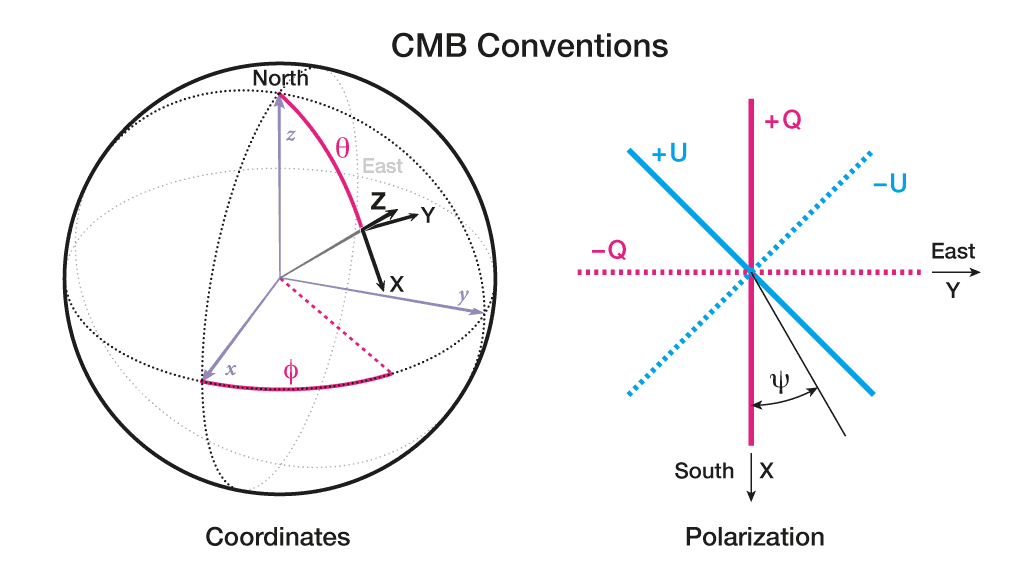
\includegraphics[width=0.7\linewidth]{figures/cmb_coord_convention}
	\caption{Figure showing the convention used for polarization among the CMB community. In this figure, $z$ is parallel to $\hat{p}_0$, $x$ is parallel to $\hat{\theta}$ and $y$ points along $\hat{\phi}$. $\psi$ is the angle between the antenna ``up'' direction, and $x$ ($\hat{\theta}$). The sign conventions of Stokes parameters $Q$ and $U$ used by the CMB community are: positive $Q$ if the polarization vector is aligned with $\hat(\theta)$ (North-South direction), negative $Q$ if the polarization vector is aligned with $\hat{\phi}$ (East-West direction), positive $U$ is aligned with $(\pm(\hat{\phi} - \hat{\theta})/\sqrt{2} )$ (North/East-South/West direction), and negative $U$ is parallel to $(\pm(\hat{\phi} + \hat{\theta})/\sqrt{2} )$ (North/West-South/East direction). Note that the right-most panel of this figure corresponds to an observer looking \textsl{towards Earth}. Figure source: \href{https://lambda.gsfc.nasa.gov/product/about/pol_convention.cfm}{LAMBDA website}}
	\label{fig::cmbcoordconvention}
\end{figure}

\section{Antenna model}
\label{sec::antennas}

\subsection{Unpolarized case}

The properties of an antenna equipped with an unpolarized receiver can be fully characterized by its beam. The antenna beam is defined in terms of its angular power density distribution $U(\rho,\sigma)$ via

\begin{equation}
\begin{aligned}
b(\rho, \sigma) = \frac{ U(\rho, \sigma) }{ \mathrm{MAX}\left[ U(\rho,\sigma) \right] }  =  \frac{ U(\rho, \sigma) }{ U(0,0) } \, .
\end{aligned}
\label{eq::beam_def}
\end{equation}

\noindent
A standard quantification of an antenna's ability to direct power to a particular region of the sky is given by the beam solid angle $\Omega$, calculated as

\begin{equation}
\begin{aligned}
\Omega = \int_{4\pi} b(\rho,\sigma) \, \mathrm{d} \Omega \, .
\end{aligned}
\label{eq::omega_def}
\end{equation}

\subsection{Polarized case: beam tensors}

A more general treatment of an antenna, that includes its polarization properties, can be obtained by combining the concept of a beam with the Mueller matrix formalism. This is a formalism by which the effect that an optical element has on the polarization state of incoming light is modeled by the multiplication of $4\times4$ matrix (a Mueller matrix) $\mathbf{M}$, with a Stokes vector $S_{\mathrm{in}}$. Using this formalism, the polarization state of light coming out of the optical element can be expressed as

\begin{equation}
\begin{aligned}
S_{\mathrm{out}} = \mathbf{M} S_{\mathrm{in}}
\end{aligned}
\end{equation}

As described in the work of \cite{piepmeier_long_njoku_2008} and \cite{2007MNRAS.376.1767O}, antennas can be modeled using Mueller matrices. PISCO is based on the work of \cite{2007MNRAS.376.1767O}, since it describes a formalism that is more suitable to be applied to CMB experiments. We note the original paper names ``beam Mueller fields'' to this extended definition of a antenna beam. In this work, we refer to it as a beam tensor, or \textsl{beamsor} for short.

A beamsor can be interpreted as a field of Mueller matrices such that for each direction $(\rho,\sigma)$, there is an associated Mueller matrix that quantifies the coupling between the antenna and a Stokes vector coming from $(\rho,\sigma)$. We will denote a beamsor by letter $B = B(\rho,\sigma)$. At every antenna basis direction, $B$ is a $4\times4$ matrix in the form

\begin{equation}
\begin{aligned}
B(\rho,\sigma) = \frac{1}{\tilde{\Omega}}
\begin{bmatrix}
B_{TT} & B_{QT} & B_{UT} & B_{VT}\\
B_{TQ} & B_{QQ} & B_{UQ} & B_{VQ}\\
B_{TU} & B_{QU} & B_{UU} & B_{VU}\\
B_{TV} & B_{QV} & B_{UV} & B_{VV}
\end{bmatrix}
\end{aligned}
\label{eq::beamsor}
\end{equation}

\noindent
where $\tilde{\Omega}$ is a normalization factor

\begin{equation}
\begin{aligned}
\tilde{\Omega} = \int_{4\pi} B_{TT}(\rho,\sigma) \, \mathrm{d} \Omega
\end{aligned}
\end{equation}

\noindent
and the elements of $B$ are defined in Appendix B. 

\subsection{Measuring the sky with antennas}

Using the formalism described in \cite{2007MNRAS.376.1767O} has the advantage of using Mueller calculus to model the process by which a detector measures the sky using an antenna. Following \cite{2007A&A...470..771J}, a partially polarized, total power detection device corresponds to the following row-vector 

\begin{equation}
\begin{aligned}
\tensor{D}{_{i}}(\zeta,\epsilon,s) = \frac{s}{2} \left[(1 + \epsilon), (1 - \epsilon)\cos(2\zeta), (1 - \epsilon)\sin(2\zeta), 0 \right]
\end{aligned}
\label{eq::M_pol}
\end{equation}

\noindent
where $1 - \epsilon$ is the polarization efficiency, $s$ is the voltage responsivity of the detector and the angle $\zeta$ is the orientation of the sensitivity axis of the linear polarizer with respect to $\hat{e}_{\co}$ at beam center. The process of taking a total power measurement on a Stokes vector $\tensor{S}{^{i}}$ is then

\begin{equation}
\begin{aligned}
d = \tensor{D}{_{i}} \tensor{S}{^{i}}
\end{aligned}
\label{eq::total_power_measurement}
\end{equation}

\noindent
Taking $\tensor{S}{^{i}}$ as the convolution between a beamsor and the sky model, a measurement taken by linearly polarized total power detector coupled to an antenna which points along $\hat{p}$ is described by

\begin{equation}
\begin{aligned}
d(\bar{q}) = \tensor{D}{_{i}}(\zeta,\epsilon,s) \int_{4\pi} \tensor{B}{^{i}_{j} } \left[ \tensor{\Lambda}{^{j}_{k} } \tensor{S}{^{k}} \right ] \, \mathbf{d} \Omega
\end{aligned}
\label{eq::total_power}
\end{equation}

\noindent
where $(i,j) = T,Q,U,V$, and $B$ has been implicitly rotated so it is aligned according to $\bar{q}$ (see Appendix A). Rotation of the sky to antenna polarization basis is carried out by $\Lambda$, which is a matrix field in the form

\begin{equation}
\begin{aligned}
\Lambda =
\begin{bmatrix}
1  & 0 & 0 & 0\\
0  & \cos(2\psi) & \sin(2\psi) & 0\\
0  &-\sin(2\psi) & \cos(2\psi) & 0\\
0  & 0 & 0 & 1
\end{bmatrix}
\end{aligned}
\label{eq::lambda_operator}
\end{equation}

%
\section{Pixel space convolution}
\label{sec::pixel_conv}

\subsection{Discrete convolution on the sphere}

It is convenient to consider a few conventions that will be used in this section. Continuous fields on the sphere are denoted using capital letters, like $F$. The $k$-th pixel of the pixelated counterpart of $F$ will be written as $\tensor[_k]{F}{}$. A useful interpretation of $\tensor[_k]{F}{}$ is to consider it as the $k$-th row in matrix of $N_p$ (number of pixels) sub-matrices. In this formalism, a pixelated beamsor would be represented by an $N_p \times 4 \times 4$ matrix.

Pixelization of a function defined on the sphere can be modeled as a process where the continuous field $F = F(\theta,\phi)$ becomes a matrix. Generally, any pixelization scheme will make use of a pixel weighting function $w(\theta,\phi)$ to smooth rapid variations of $F$ inside the pixel domain. This is crucial to avoid aliasing noise, which can negatively impact harmonic space analysis of pixelated maps. In this context, to obtain the value of $\tensor[_k]{F}{}$ we must calculate the convolution of $k$-pixel weighting function with $F$, namely 

\begin{equation}
\begin{aligned}
\tensor[_k]{F}{} = \int {}_k w (\theta,\phi) F(\theta,\phi) \, \mathrm{d} \Omega
\end{aligned}
\label{eq::howtopixelate}
\end{equation}

\noindent
It is worth noting that PISCO does not explicitly compute equation \ref{eq::howtopixelate}, as the input maps which are used to generate TOD are already pixelated. The same situation applies for beamsors, which are also inputted as pixelated maps.

Following the aforementioned conventions, the pixel space version of equation \ref{eq::total_power} becomes

\begin{equation}
\begin{aligned}
d(\bar{q}) = \
\tensor{D}{_{i}}(\zeta,\epsilon,s) \
\sum_{k=1}^{N_p} \
\tensor[_k]{B}{^i_j} \
\tensor[_k]{\Lambda}{^j_m} \
\tensor[_k]{S}{^m}
\end{aligned}
\label{eq::discrete_beam_conv_tensor}
\end{equation}

\noindent
where we have implicitly assumed that $B$ has been properly re-pixelated so as to be aligned according to $\bar{q}$. 

\subsection{Implementation in CUDA}

GPUs allow for substantial acceleration of algorithms that perform a large amount of independent operations\cite{sanders2010cuda}. TOD generation using equation \ref{eq::discrete_beam_conv_tensor} is a great application case, because all operations are independent of each other, including the ones within a convolution. To better understand how this parallelism can exploited, consider the process of synthesizing $N_s$ measurements, each one associated with a pointing $\bar{p}_t$, using a CUDA grid of $B$ blocks and $T$ threads.

The main algorithm consists of two nested loops, $L1$ and $L2$. $L1$ loops over the pointing, so that each block is associated with a given pointing direction. Note that this makes $L1$ execute $B$ operations in parallel. To prevent a race condition, the pointing is cloned $T$ times so that each thread in a block can read it from memory as fast as possible. $L2$ iterates on beamsor and sky pixel. Since every block executes $T$ threads, every block can compute $N_p/T$ partial summations of equation \ref{eq::discrete_beam_conv_tensor} in parallel. A third, higher level loop, can also be added to the algorithm to further chunk the pointing stream and make use of $N_g$ GPU instances. A graphical description of the algorithm is shown in figure \ref{fig::pisco_diagram}.

\begin{figure}
	\begin{center}
		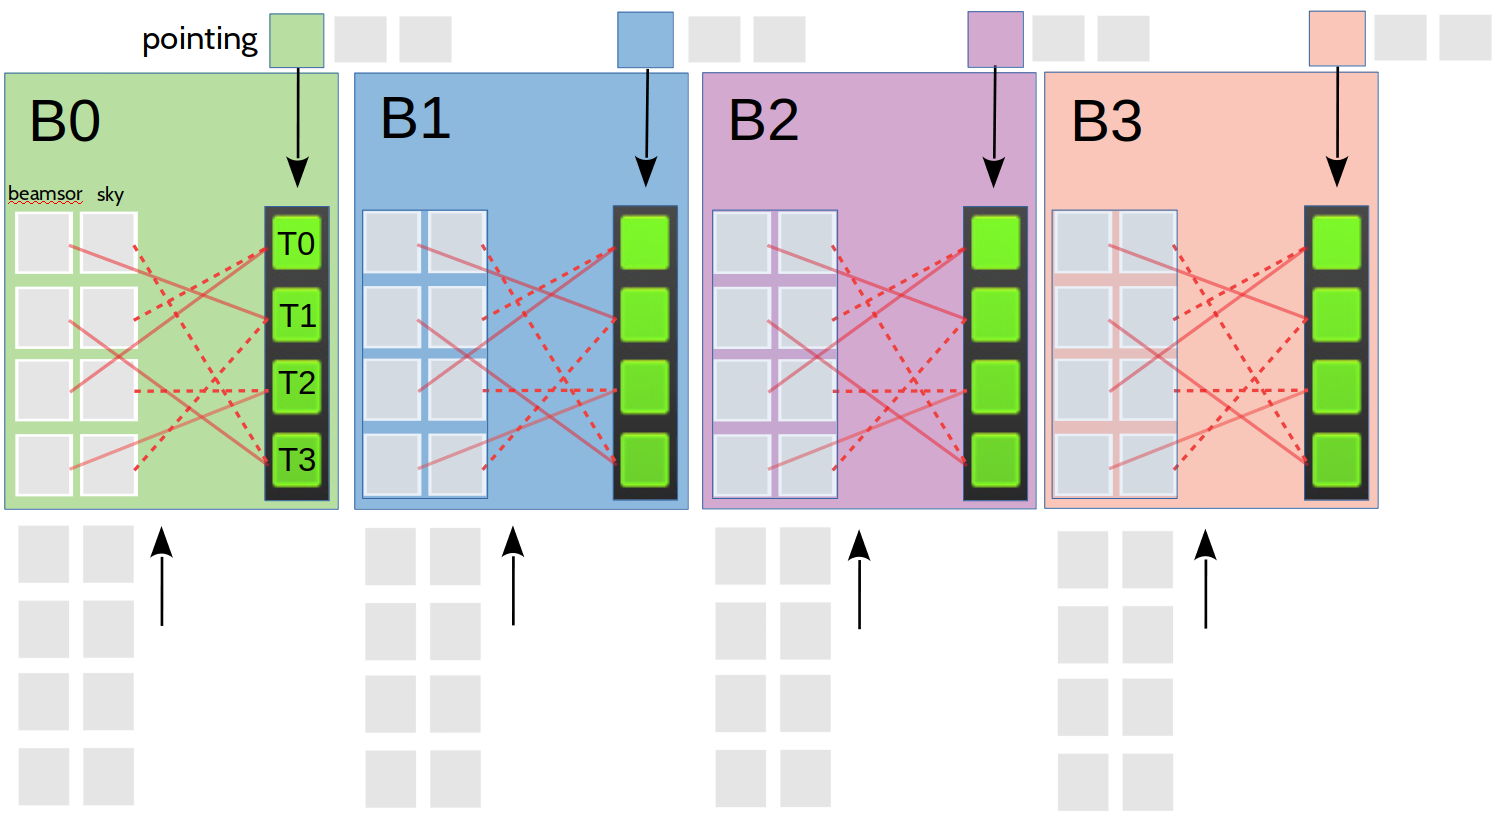
\includegraphics[width=0.8\linewidth]{figures/PISCO-diagram.png}
		\caption{Parallelization scheme. This figure shows the case of PISCO executing in 4 blocks ($B=4$), with four threads per block ($T=4$). Arrays with beamsor and sky elements are at the bottom. Each block has access to four beamsor and sky pixels (gray boxes inside colored boxes) and one pointing entry (colored small boxes) at a time. Green boxes represent the multiplication process of a single beamsor pixel with a single sky pixel. This includes rotating the sky pixel to the antenna polarization basis, and computing the repixelization of $B$ at the corresponding coordinates. Solid and dotted red lines represent the complex memory access pattern generated by this process. Every thread within a block writes its result to shared memory space. When a thread finishes its computation, it waits until all threads have finished and a reduction on the shared memory space is performed on across all blocks. This process is repeated for every pointing. At the end of the procedure, each block has computed the convolution of a beamsor with the sky for a particular pointing, and every shared memory space of the block has the corresponding result. These results are collected into the GPU global memory, which is then transferred back to CPU (host) memory.}
		\label{fig::pisco_diagram}
	\end{center}
\end{figure}

\subsection{PISCO}

The \textbf{PI}xel \textbf{S}pace \textbf{CO}nvolver (PISCO) is a tool with the capability of generating synthetic Time Ordered Data (TOD) provided a model for the beamsor, the scanning strategy of the mission and a sky model. In this section, we present a pathfinder implementation of PISCO that makes use of the massively parallel architecture of modern GPU systems.

\subsubsection{General description}

PISCO is the software tool in charge of generating mock TOD given a beamsor, a sky model and a scanning strategy. A diagram showing the general workings of PISCO is shown in figure \ref{fig::pisco_flow}. PISCO receives as input a sky model in the form of 4 maps representing Stokes parameters $I,Q,U$ and $V$, a beamsor, pointing and focal plane information. The focal plane specifications are only needed if multiple detectors are being included in the pointing stream, as PISCO needs the the angle $\zeta$ of each detector to compute equation \ref{eq::discrete_beam_conv_tensor}. All the inputs are sent to the TOD generation function, which returns the data streams. At this point, the data can either be saved to disk or sent to a map-making code. This last step is preferred as, usually, input-output operations are time consuming. Finally, maps can be analyzed using external tools to calculate the power spectra.

\begin{figure}
	\centering
	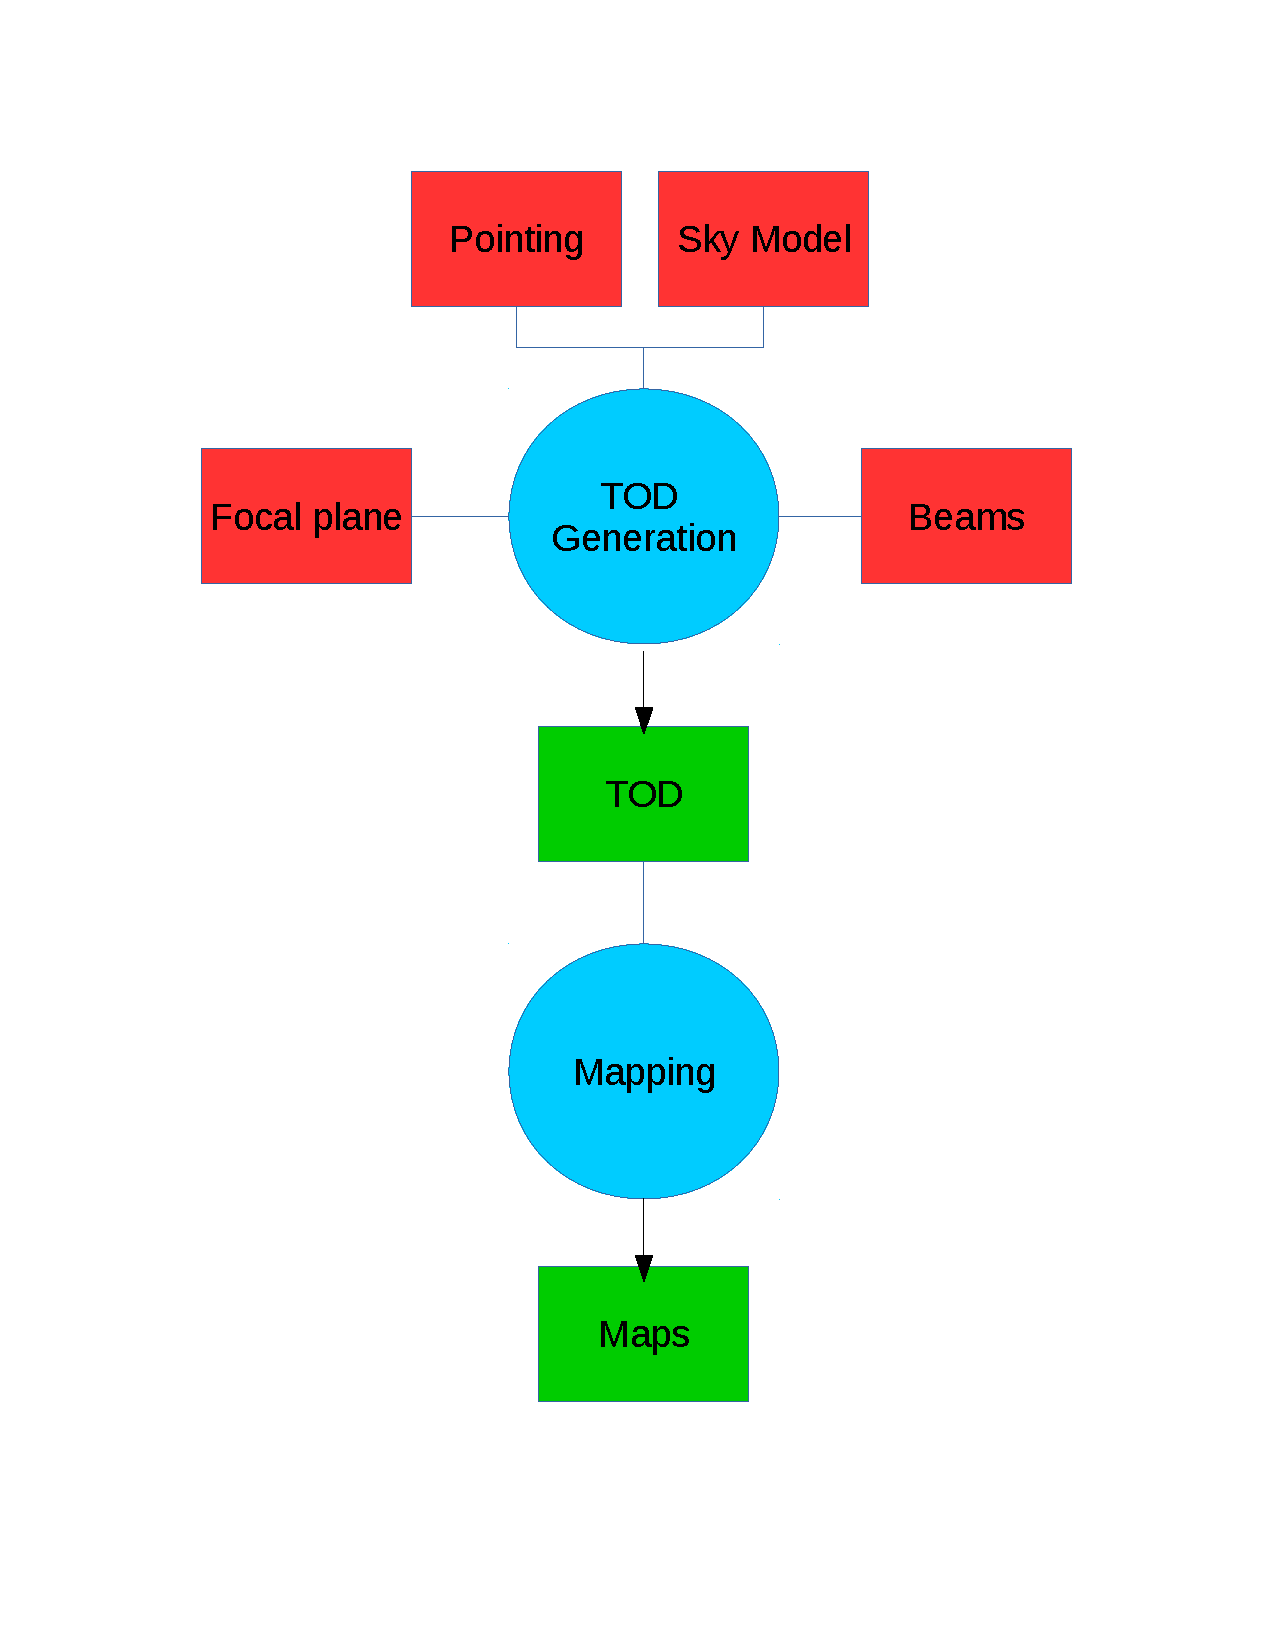
\includegraphics[width=0.6\linewidth]{figures/pisco-flow-diagram}
	\caption{Basic flow of a typical PISCO simulation pipeline. Red polygons show the required user input. PISCO uses this input and produces TOD (green polygon). This TOD stream is calculated using equation \ref{eq::discrete_beam_conv_tensor} for all pointing directions. TOD can then by sent into a mapper and, finally, to a power spectra estimator tool. PISCO does not compute pointing nor produces maps from TOD by itself; these tasks are left to external programs.}
	\label{fig::pisco_flow}
\end{figure}

\subsubsection{Performance}

For large enough pointing streams, the available parallelism scales as $N_g \times B \times T$. We note that using larger pointing streams might affect performance, as reading from disc is usually slow. We believe that this penalty should be greatly suppressed by the use of a parallel file-system, which is a standard capability of modern HPC facilities. We also performed a test showing that the time spent loading a pointing stream with over 870 million data points takes less than $1\%$ of the overall execution time. Following the experience of FeBeCOP and TOAST, the current pipeline shown in figure \ref{fig::pisco_flow} does not write the mock TOD to disc.

A realistic run took about 4 hours and 10 minutes on a single NVIDIA GTX 1080. The machine was also equipped with two Intel Xeon E5-2610 processors (20 physical cores, 40 threads). This run generated mock data for more than 870 million pointing directions. Each beamsor was represented by 5940 pixels. We note that this number only increases the accuracy of the re-pixelization step at the cost of increased memory requirements rather than any additional compute time. The actual number of pixels involved in a single convolution was 370 on average. The time taken by the map-making code is negligible compared to the convolution step, so it is not considered. With this particular simulation setup, PISCO was able to generate data 40 times faster than a real-time observation by computing more than 19 million convolutions per second. 

The complex operations in the CUDA kernels involve large amounts of floating point and integer computations. This makes it difficult to estimate the performance as FLOPS. Also, the CUDA routine reads values from memory in a pseudo-random access pattern, something that is not efficiently performed by GPUs. The penalty associated with this situation is challenging to estimate. Finally, this implementation of PISCO pre-computes the cap of pixels around a given pointing direction in the CPU. While this process is fast, transferring the resulting memory buffer to the GPU takes as much as $30\%$ of the computation time. A solution to this problem has already been devised, and will be implemented in future releases.

\begin{table}[tbp]
	\centering
	\begin{tabular}{|c|c|c|}
		\hline
		Routine description & Time (in seconds) & $\%$ of total time \\
		\hline
		convolution & 7967 & 52$\%$  \\
		query pixel cap & 2171 & 14$\%$ \\
		transfer pixel cap & 3978 & 27$\%$ \\
		others & 985 & 7$\%$ \\ 
		\hline
	\end{tabular}
	\caption{Table summarizing the times taken by different routines of PISCO. The simulation executed at more than 19 million convolutions per second.}\label{tbl1}
\end{table}

%
\section{Code validation}
\label{sec::validation}

To validate the correctness of PISCO, we performed two sets of tests: a mock observation of a (polarized) point source and a simulation of an ideal CMB observation. All simulations were performed in a machine equipped with three NVIDIA GTX 1080 cards, two Intel Xeon E5-2610 processors (20 physical cores, 40 threads) and $256$ GB of RAM. 

Results from these tests were compared against the \texttt{healpy.smoothing} routine, a Python wrapper around HEALPix routines (see \cite{2005ApJ...622..759G}), which calculates the convolution of a polarized sky with a circularly symmetric Gaussian beam in $a_{\ell m}$ space. For the purposes of this section, we will consider the output of \texttt{smoothing} to be exact. 

\subsection{Point source observations}

The simulated observation of a polarized point source was accomplished by the following steps

\begin{itemize}
	\item Build a beamsor without cross-polarization Each $M_{ii}$ component is a circular Gaussian beam with FWHM of $1.5^\circ$.
	\item Build a $I,Q$ and $U$ skies with a single non-zero pixel at coordinates $(\theta_k,\phi_k)$ The Stokes parameters $S^{i} = (1,Q,U,0)$ of the pixel are set such that $Q^2 + U^2 = 1$.
	\item Set up a raster scan around $(\theta_k,\phi_k)$ for a detector with $\zeta=0$. Note that, in order to have full polarization coverage, the raster scan is repeated 3 times with angles $\psi_0 = 0^{\circ},45^{\circ},90^{\circ}$.
	\item Make maps of TOD generated by PISCO.
	\item Compare the result of applying \texttt{smoothing} to the single pixel map using the same beam model.
\end{itemize}

\subsubsection{Results}

Results from this validation test are shown in figure \ref{fig::stokesqsource256beam1024dec45}. The results show that the flux is preserved to better than $0.1\%$. Using a lower \texttt{NSIDE} for the beamsor degrades this considerably. We checked for systematic effects driven by the finite machine precision of the computations, and found that leakage from temperature to polarization is least $10$ orders of magnitude below the maximum amplitude of the Stokes I convolved map. PISCO is also able to correctly account for intra-beam variations of the position angle $\psi$.

\begin{figure}
	\centering
	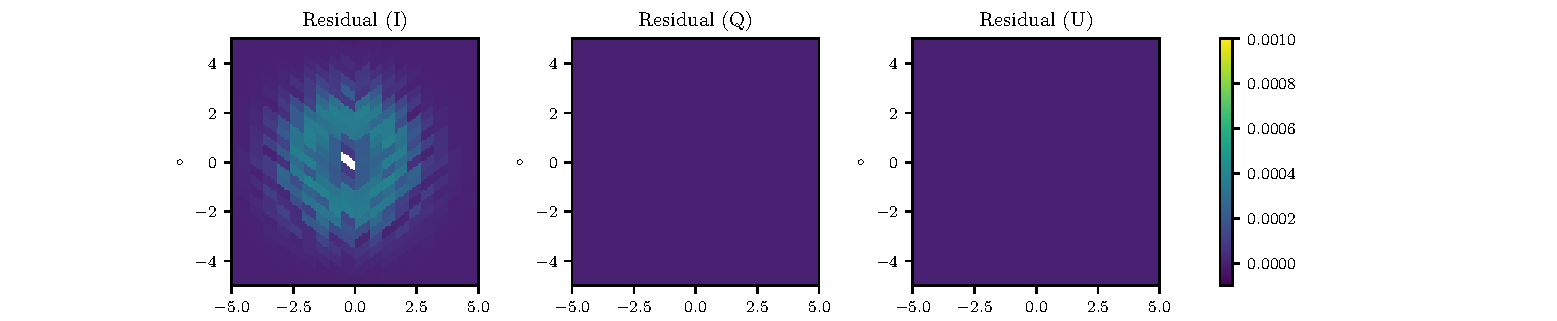
\includegraphics[width=1.0\linewidth]{figures/stokes_I_source_256_beam_1024_dec_45.pdf}
	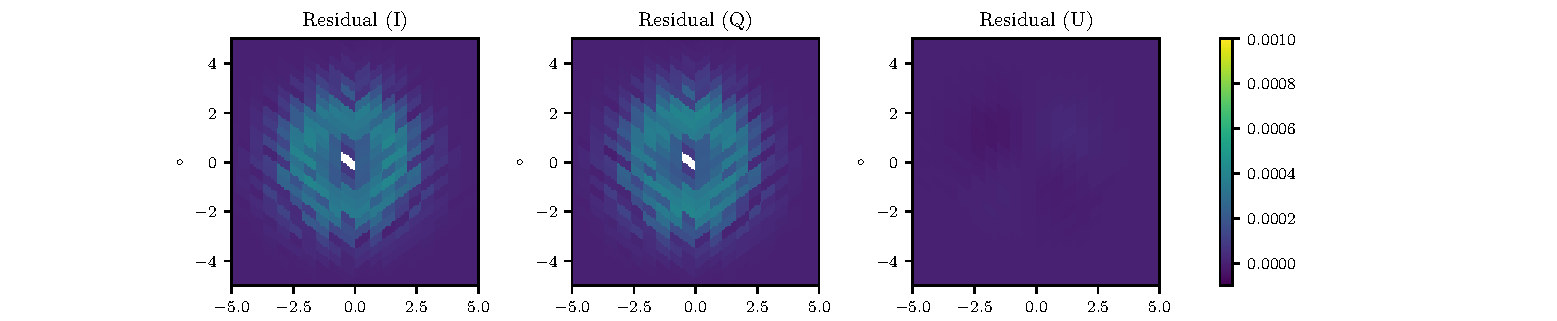
\includegraphics[width=1.0\linewidth]{figures/stokes_Q_source_256_beam_1024_dec_45.pdf}
	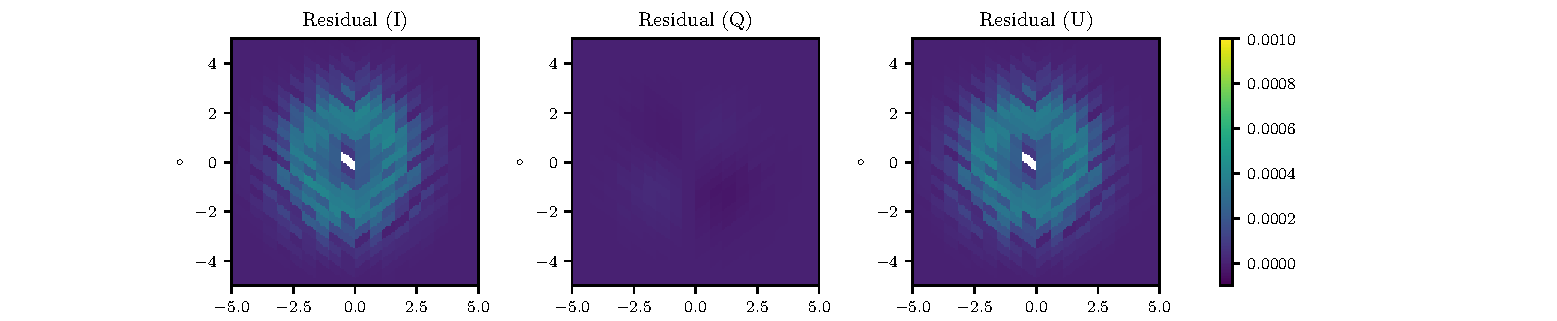
\includegraphics[width=1.0\linewidth]{figures/stokes_U_source_256_beam_1024_dec_45.pdf}
	\caption{Figure showing the results from subtracting a map of a point source convolved with a Gaussian beam using \texttt{smoothing}, and the map using generated by PISCO. Input map used HEALPix pixelization with $\mathrm{\texttt{NSIDE}} = 256$. Beamsor uses $\mathrm{\texttt{NSIDE}} = 1024$. Gaussian profile used for the beamsor had a FWHM of $1.5^\circ$. All point sources are located at $45^\circ$ declination. Color scale is normalized to $1$. From top to bottom: residuals for the case of a point source with Stokes vector $S = (1,0,0,0)$, $S=(1/\sqrt{2},1/\sqrt{2},0,0)$ and $S=(1/\sqrt{2},0,1/\sqrt{2},0)$, respectively.}
	\label{fig::stokesqsource256beam1024dec45}
\end{figure}

\subsection{Ideal CMB experiment}
\label{sec::ideal_full_sky}

\subsubsection{Description}

Similarly for the point source observation, the simulating an ideal CMB experiment was accomplished by following

\begin{itemize}
	\item Build a beamsor without cross-polarization Each $M_{ii}$ component is a circular Gaussian beam with FWHM of $1.5^\circ$.
	\item Build mock CMB whole sky maps with a tensor-to-scalar ratio $r=0.0$.
	\item Set up a scanning strategy to visit each pixel center at 3 different position angles $\psi_0 = 0^{\circ},45^{\circ},90^{\circ}$. 
	\item Make maps of TOD generated by PISCO. 
	\item Compare the maps with a harmonic space convolution of the CMB map with a Gaussian beam.
\end{itemize}

\subsubsection{Sky model}

Input sky maps were generated using a combination of CAMB (see \cite{Lewis:2002ah}) to generate $C_\ell$ and \texttt{synfast} The cosmological model was set to complain to the latest results of the Planck satellite (see \cite{2016A&A...594A..13P}). This procedure returns 3 CMB anisotropy maps, one for each Stokes parameter\footnote{It is usually assumed the CMB has no circular polarization, so $V$ map was set to zero.} CAMB was configured to return a CMB with no primordial B-modes ($r=0$) and no lensing, as this last effect is expected to produce leakage from E-modes to B-modes. The resulting B-mode power spectrum is effectively zero at all angular scales. No foreground or other sources were added on top of the simulated CMB. All maps use the \texttt{HEALPix} pixelization and were generated at a resolution of \texttt{NSIDE}$=128$. This restricts the analysis in harmonic space to $\ell < 384$.

\subsubsection{Scanning strategy}

The scanning strategy was designed so that every pixel on the sky gets visited exactly three times, each one at a different beam orientation angle. In addition, every pixel is observed at its center, which is an important requirement that ensures the intra-pixel coverage does not affect the estimation of the power spectra at high $\ell$. Since only three hits per pixel at different values of $\psi$ are required to recover the polarization field of the CMB, the scanning was generated for a single detector with a polarization sensitive angle $\zeta=0$.

\subsubsection{Power spectra}

Power spectra was calculated using \texttt{anafast}. No further post-processing of the power spectra was needed given that this simulated observation covers the whole sky, and hence no masking effects arise. The power spectra corresponding to maps that were generated using PISCO TOD were corrected by the equivalent beam transfer function of a circular Gaussian beam of FWHM$=1.5^\circ$. 

\subsubsection{Results}

Results are shown in figure \ref{fig::pisco4wholesky}. We found there is excellent agreement between the output of \texttt{smoothing} and PISCO, with little or no signs of significant deviations across the $\ell=[2,250]$ span. 

include the temperature power spectrum.
include a power spectra residual plot.

\begin{figure*}
	\centering
	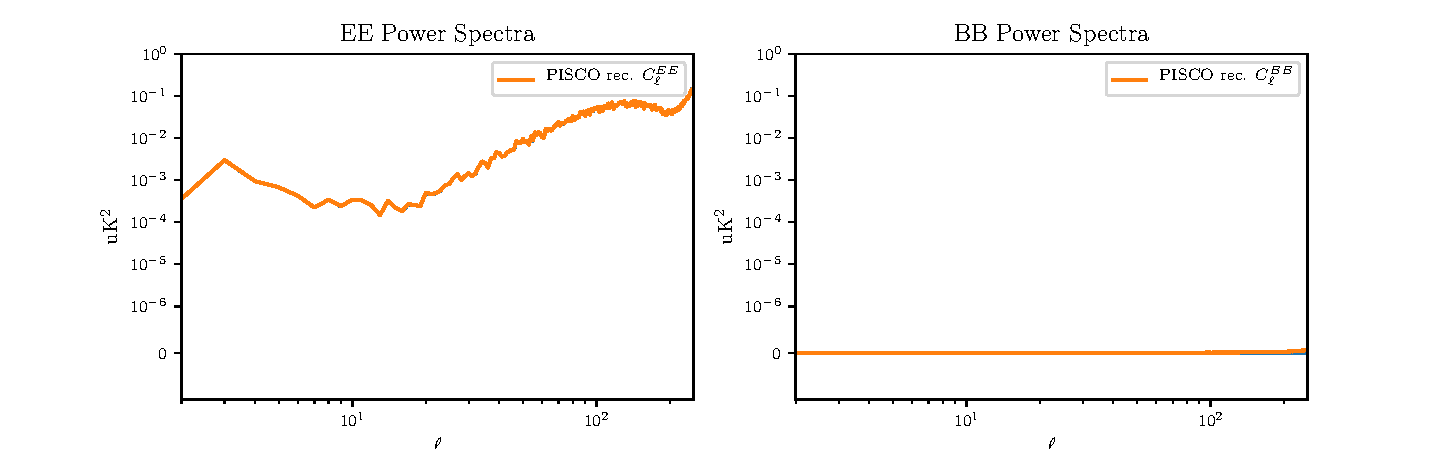
\includegraphics[width=1\linewidth]{figures/ps_r0d00.pdf}
	\caption{Plots showing maps of PISCO generated TOD and the results from \texttt{smoothing} for whole sky CMB test. Top plot corresponds to power spectra of the input map (blue circles) and the output of PISCO (orange curve) Bottom plot corresponds to the residuals between the input power spectra the one computed from maps generated using PISCO.}
	\label{fig::pisco4wholesky}
\end{figure*}

%
\section{Realistic CMB experiment}
\label{sec::realistic_cmb_experiment}

In this section, we describe the procedure and results of a more realistic simulation of a CMB experiment using PISCO. Designing a such an experiment from scratch is a challenging task, so we based the simulation on an ongoing mission, the Cosmology Large Angular Scale Surveyor, CLASS\cite{2016SPIE.9914E..1KH} CLASS aims at characterizing the CMB polarization anisotropy field at large angular scales, particularly the B-mode power spectrum, looking for signatures that could indicate Inflation took place. While the experiment is composed of 4 telescopes, the simulation focuses on the one observing at the lowest frequency (38 GHz), the Q-band receiver. This decision was taken for computational reasons: generating TOD using PISCO scales linearly with the number of detectors and with the length of the pointing stream. Given that CLASS aims at measuring the sky signal over the whole celestial sphere, simulating a receiver with less extended beams requires sampling a higher resolution map than the case of a wide beam. In consequence, the pointing stream must include more samples so as not to get missing pixels. Similarly, higher frequency receivers have in the order of 500 detectors, while the Q-band receiver only has 72. The combination of less detectors with larger beams makes CLASS and its Q-band receiver a good application case to check if PISCO is able to simulate a CMB experiment, using a high-end workstation instead of an HPC facility. 

\subsection{Description}

\subsubsection{Sky model}

To generate the maps for this simulation, we followed a similar procedure to the one described in section \ref{sec::ideal_full_sky}. The main difference is the addition of an unpolarized CMB, which was used to check for  T to P leakage caused by effects not present in the test described in the previous section. All maps use the \texttt{HEALPix} pixelization and were generated using \texttt{NSIDE}$=128$. 

\subsubsection{Pointing}

The scanning strategy of CLASS consists of constant elevation scans (CES). Elevation is kept at $45^{\circ}$ while the telescope rotates $720^\circ$ in azimuth at $1$ degree per second. This process is repeated for around 18 hours per day. The boresight is rotated from $-45^{\circ}$ to $+45^{\circ}$ by $15^{\circ}$ per day on a weekly schedule. This scanning strategy, in combination with the large CLASS Field Of View (FOV) makes the telescope cover more than 70 percent of the sky every 24 hours. In addition, because of the boresight rotation, only seven days are needed to provide excellent position angle coverage. Boresight rotation is also key to allow modulation of both $Q$ and $U$ signals (see \cite{2016SPIE.9914E..1KH}) While CLASS records data $200$ times per second, the pointing streams were generated at $20$ Hz. This down-sampling factor was selected so as not to produce pixel misses, with the median number of hits per pixel is being in the order of thousands (PF check this with the plots from mapstats). Down-sampling allows for a ten-fold decrease in computation time.

Taking into account the above considerations, the boresight pointing was generated by closely emulating the scanning strategy in horizontal coordinates (constant elevation scans). Next, the equatorial coordinates for every detector on the focal plane were calculated using from this stream and the beam center offsets of every detector. We note that this procedure does not take into account telescope down-time caused by daily maintenance or other systematic effects, like variations on the pointing model. The scanning strategy that was used for this simulation corresponds to seven continuous streams of 24 hours, one for each boresight angle, sampled at $20$ Hz. The pointing stream has more than 870 million individual directions. 

\subsubsection{Beamsor model}

Following the work of \cite{2012SPIE.8452E..20E} and valuable input from the CLASS Collaboration, beamsor models for all 72 detectors of the Q-band receiver were built. For simplicity, beam tensors do not include any cross-polarization, while the two dimensional profile of the diagonal elements correspond to purely elliptical Gaussian profiles. The simplicity of the beams allows for a further speed-up in the computation by restricting the convolution to a $5^\circ$ disc around the beam center. This value was chosen as, for a unit normalized Gaussian beam, a pixel that is $5^\circ$ away from the centroid has a value of $\approx 10^{-14}$, roughly the limit of double precision arithmetic. Beamsors were also projected into a HEALPix grid of NSIDE=512, which produces an error in the simulated TOD of less than $0.01\%$.

%\begin{figure}
%	\centering
%	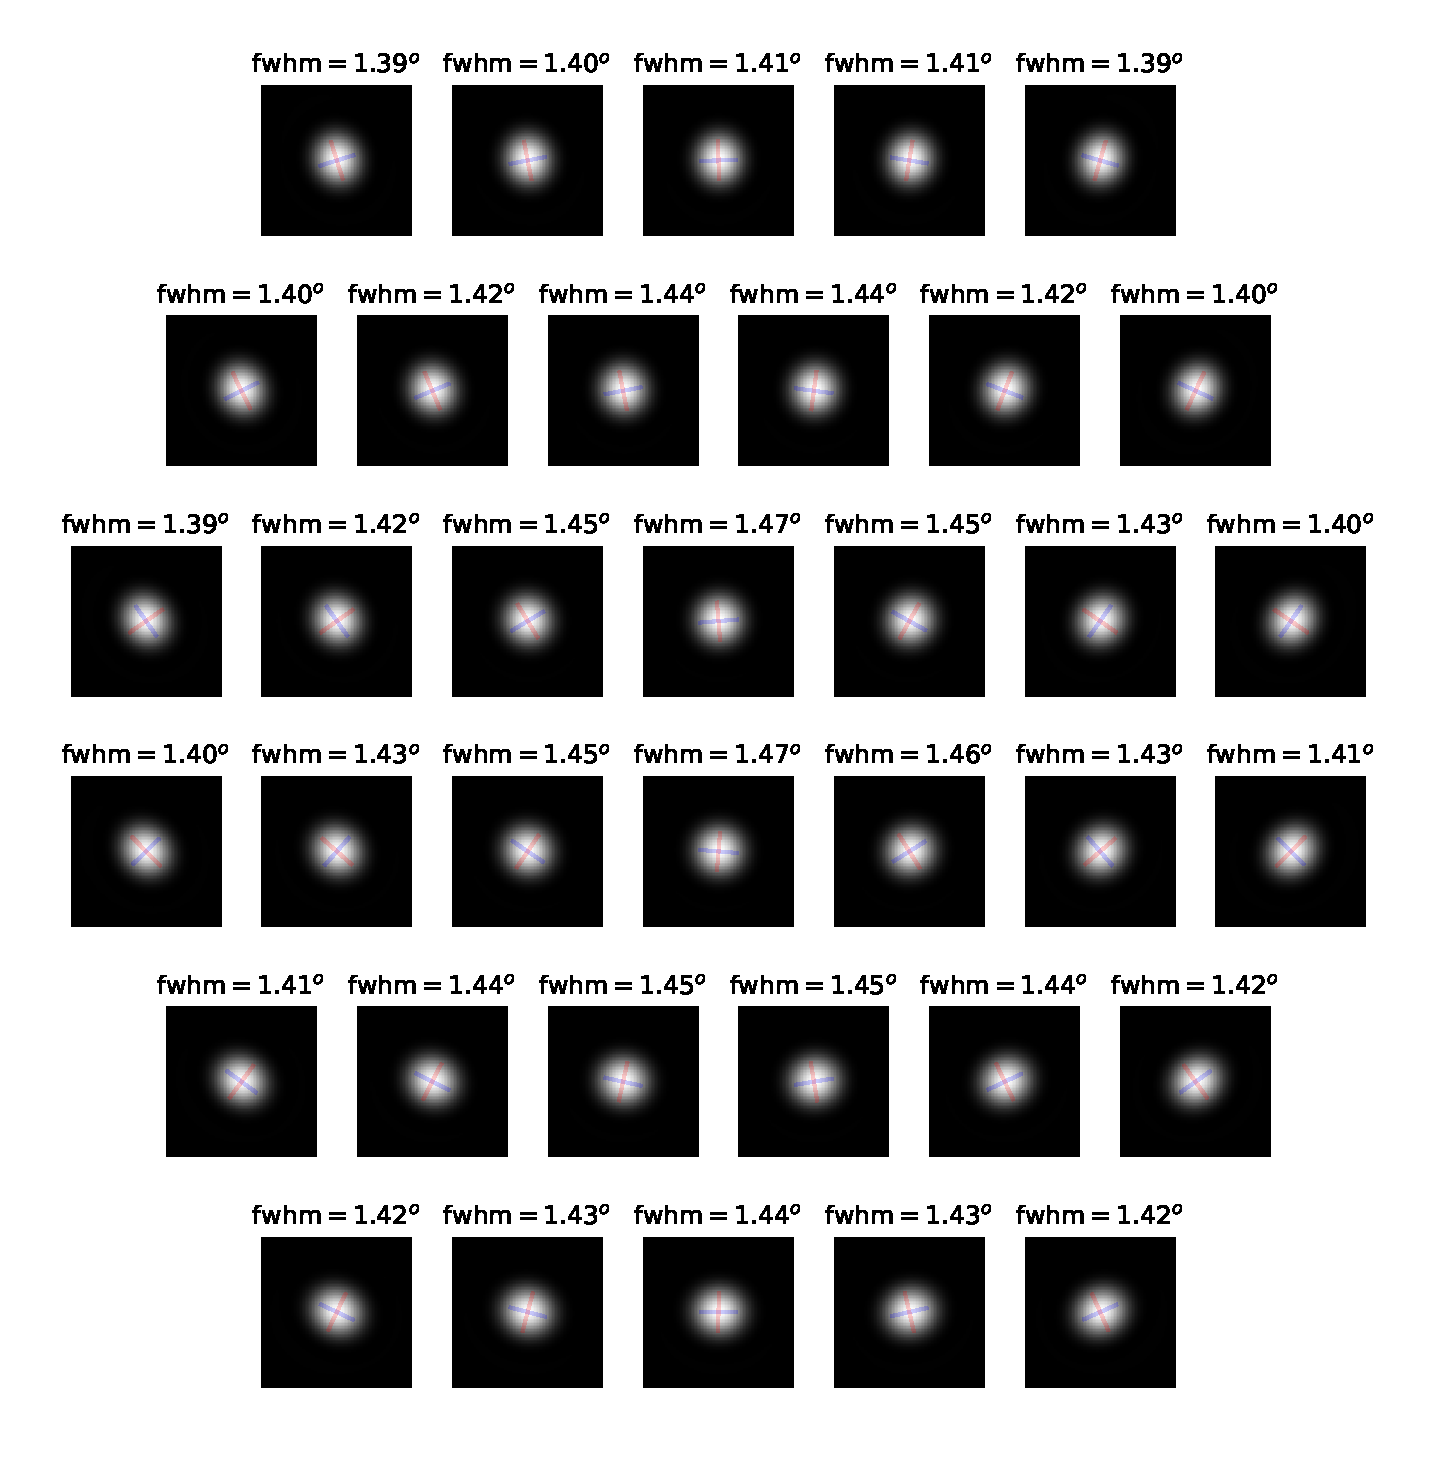
\includegraphics[width=0.8 \linewidth]{figures/qband_beams_main_beam_fwhm_x}
%	\caption{Elliptical Gaussian profiles used as beamsor models for the CLASS Q-band telescope. Relative positions of plots are representative of the positions of feedhorns on the sky. In image coordinates, Zenith is up while East is to the left. All beam profiles are unit normalized, the color scale being linear. Each subplot is a plane projection on the sky of $5^\circ \times 5^\circ$. The title of each subplot is the Full Width at Half Maximum of the profile along its semi-major axis. Non negligible amounts of eccentricity can be seen in the beam profiles, and a visible correlation between beam location on the sky, beam eccentricity and orientation of the major (minor) axis is present. Maximum eccentricity reaches $0.45$ for edge beams.}
%	\label{fig::qbandbeamsmainbeamfwhmx}
%\end{figure}

\subsubsection{Power spectra and beam transfer function}

Given that CLASS only covers $\approx 75\%$ of the sky, computing the power spectra of simulated maps requires the use of an estimator than can handle a mask. For this reason, we changed the estimator to \texttt{PolSpice} (PF cite polspice). In addition, the CLASS collaboration provided a realistic sky mask that also covers the galactic plane. 

PF write a description of the method used for the window function in the case of several elliptical beams

\subsection{Results}

\subsubsection{Effect of pointing mismatch}

In this section were refer to pointing mismatch to the difference between beam center offsets for pairs of detectors belonging to the same feed. The work of (cite Bicep paper here and others) shows that pointing mismatch can produce leakage from temperature to polarization. The goal of this section is to show that PISCO can reproduce this behavior. Two tests were performed to address this; the first test simulates the CLASS Q-band receiver scanning an unpolarized CMB with matched beams and pointing, while the second test introduces a pointing mismatch while keeping other conditions the same. The amplitude of this mismatch comes from preliminary results of the CLASS Q-band receiver. 

\begin{figure*}
	\centering
	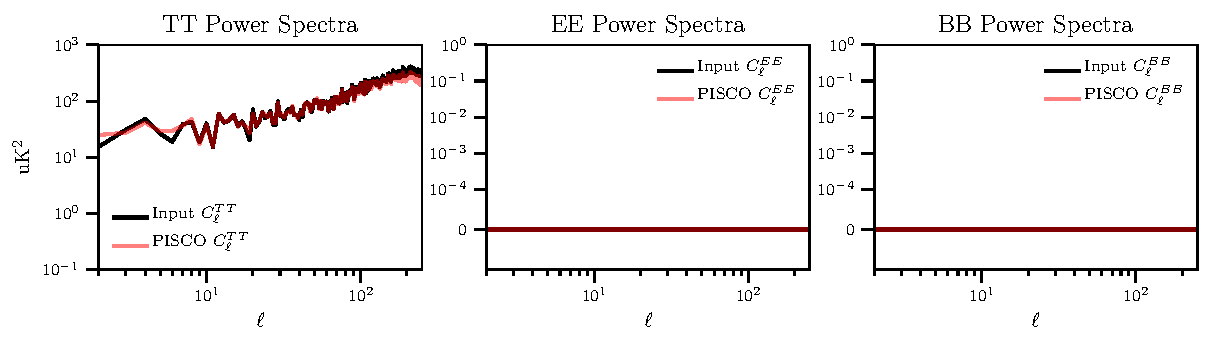
\includegraphics[width=1\textwidth]{figures/unpolCMB_r0d00_CLASS_matchedPointing_matchedBeams_ellipticalBeams.pdf}
	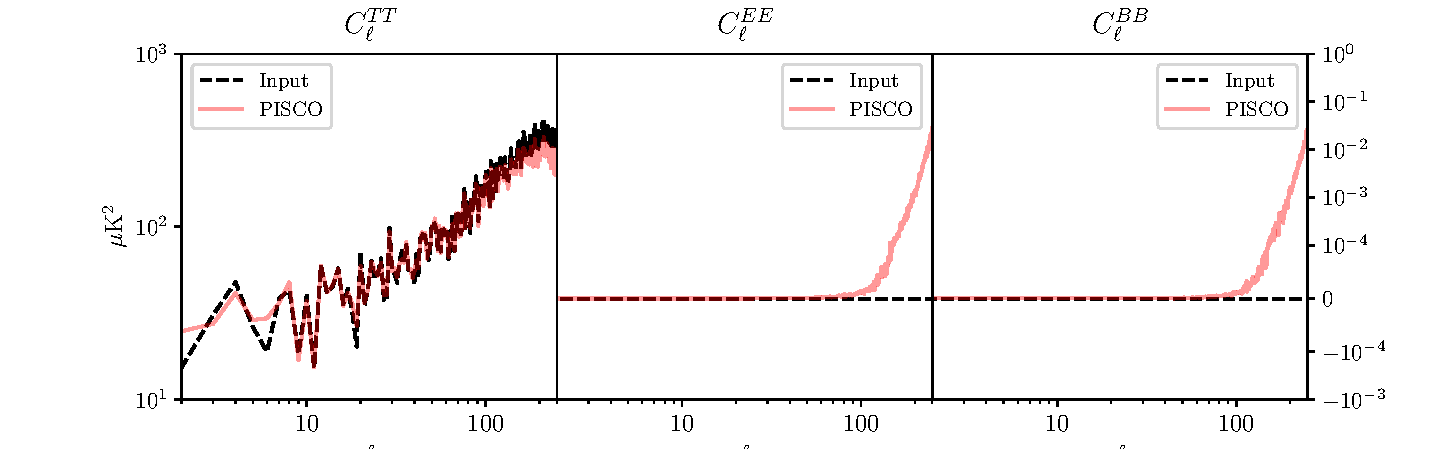
\includegraphics[width=1\textwidth]{figures/unpolCMB_r0d00_CLASS_mismatchedPointing_matchedBeams_ellipticalBeams.pdf}
	\caption{Plots power spectra for the case of matched pointing (upper figure), and mismatched pointing (bottom figure). Significant leakage from $TT$ to $EE$ and $BB$ power spectra is present for the case of mismatched pointing, reaching in the order of $100$ nK at $\ell = 250$.}
	\label{fig::pisco4class_pointingmismatch}
\end{figure*}

\subsubsection{Effect of uneven intra-pixel coverage}

Simulating a CMB experiment using a more realistic scanning strategy can produce another systematic effect at the power spectra level. This source of noise is related to the intra-pixel coverage of the observed pixels. In section \ref{sec::ideal_full_sky}, all pixels were observed exactly at their centers while, in a real experiments, every sample of the TOD ``hits'' a given pixel at an arbitrary location. If, in average, the distribution of hits inside a pixel is symmetric with respect to pixel center coordinates, map-making will average all observations and the power spectra from the resulting map will not be affected. However, if this distribution is asymmetric, the resulting maps will produce P to P leakage on the power spectra, as discussed in (Poutanen et al. 2004) and \cite{2005poutanen}. 

In this section, we aimed at exploring this effect for the CLASS Q-band receiver by repeating the simulation performed in the above section, this time using a polarized CMB as input. It is worth mentioning that the input CMB has no primordial B-modes and no E-mode to B-mode leakage caused by lensing, so that any resulting B-mode signal must be the result of leakage. Based on the results of the previous test, we can argue that uneven intra-pixel coverage causes leakage from P to P. As it was shown in the previous section, PISCO does not cause leakage when simulating the observation of an unpolarized CMB when both pointing and beams are matched. In the case of pointing mismatch, T to P leakage occurs. Conversely, this test shows that even in the case of matched beams and matched pointing, the resulting B-mode power spectrum diverges at high $ell$. Since this signal is not caused by T to P leakage (see Figure \ref{fig::pisco4class_pointingmismatch}), the only option is that it is P to P type. We note that this systematic effect is subdominant with respect to T to P leakage caused by pointing mismatch. 

\begin{figure*}
	\centering
	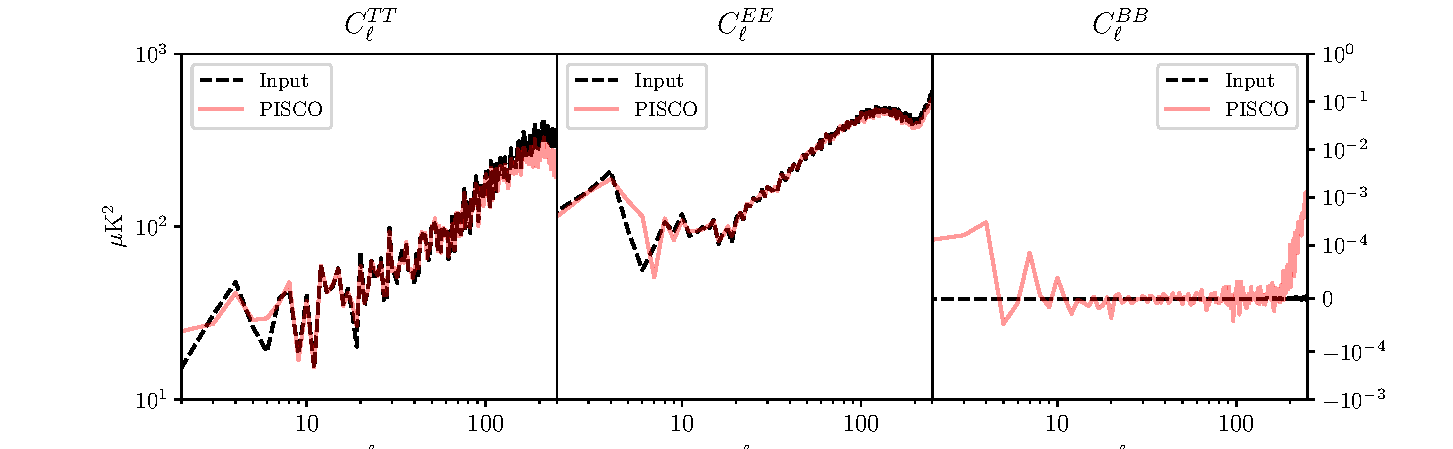
\includegraphics[width=1\textwidth]{figures/cmb_r0d00_CLASS_matchedPointing_matchedBeams_ellipticalBeams.pdf}
	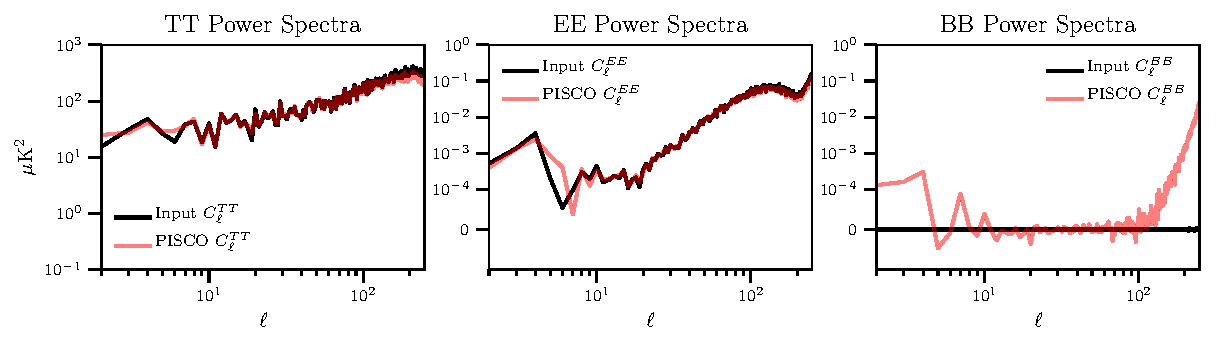
\includegraphics[width=1\textwidth]{figures/cmb_r0d00_CLASS_mismatchedPointing_matchedBeams_ellipticalBeams.pdf}
	\caption{Plots power spectra for the case of matched pointing (upper figure), and mismatched pointing (bottom figure), using a polarized CMB as input. Both figures show non-negligible amounts of leakage, which shows up as a non-zero B-mode power spectrum. In the case of matched pointing, this leakage is roughly an order of magnitude less ($10$ nK) than the case of matched pointing (100 nK) at $\ell = 250$.}
	\label{fig::pisco4class_pointingmismatch}
\end{figure*}

%
%If an experiment has a focal plane with detector pairs in the same feed, the map-making will naturally pair difference the signals. If there is a pointing mismatch, leakage from temperature to polarization (cite this) Similarly, beam mismatch within pairs can produce polarization to polarization leakage. 
%
%\begin{figure}
%	\centering
%	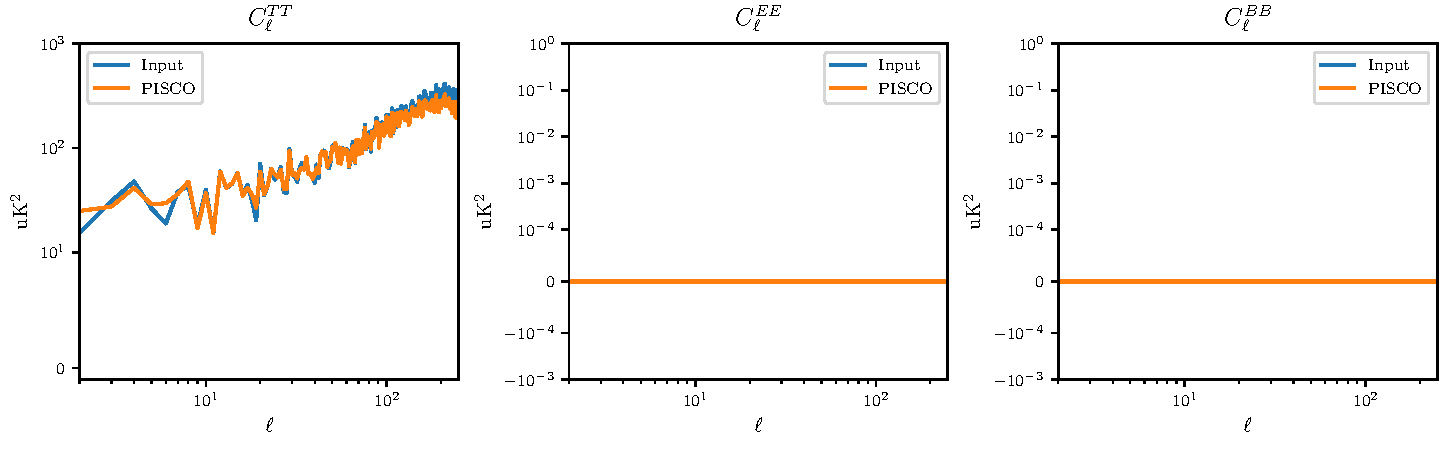
\includegraphics[width=1.0\linewidth]{figures/unpolCMB_r0d00_CLASS_matchedPointing_mismatchedBeams_ellipticalBeams.pdf}
%	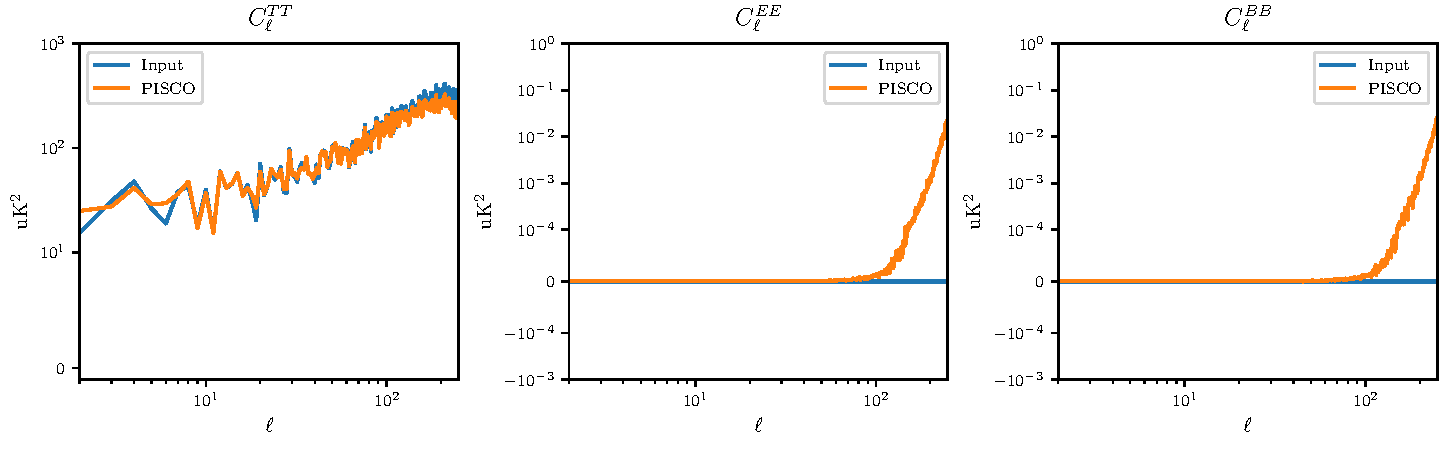
\includegraphics[width=1.0\linewidth]{figures/unpolCMB_r0d00_CLASS_mismatchedPointing_mismatchedBeams_ellipticalBeams.pdf}
%	\caption{Upper plot. Run using an unpolarized CMB as input. Focal plane has matched pointing for all pairs. Pointing was generated so as to emulate the CLASS scanning strategy. Beams follow elliptical Gaussian profiles, and are mismatched between pairs of detectors. This figure shows that even in the presence of mismatched beams, T to P leakage does not occur. Bottom plot: similar conditions to the ones used to generate the plot above, but using \textsl{mismatched} pointing at the focal plane (as well as in the pointing stream). T to P leakage does occur in this case, reaching a maximum of $\approx 50$ nK at $\ell = 250$.}
%	\label{fig::unpolcmbr0}
%\end{figure}

%
%According to literature, building a map from TOD that doesn't provide symmetric intrapixel coverage can produce divergence on the power spectra at high $\ell$. This effect becomes more dominant for the polarization power spectra, as the signal is amplitude is lower (see Hivon et al, 2002, etc), and can be interpreted as P to P leakage. For this run, we used matched beams for detectors within a pair by averaging the parameters beam pair parameters (FWHMs and ellipse rotation). Using matched beams eliminates the expected P to P leakage associated with this condition. According the Figure \ref{fig::unpolcmbr0}, the only sources of leakage in this experiment should correspond to T to P leakage arising from mismatched pointing, as well as P to P leakage caused by asymmetric intrapixel coverage. 
%
%\begin{figure}
%	\centering
%	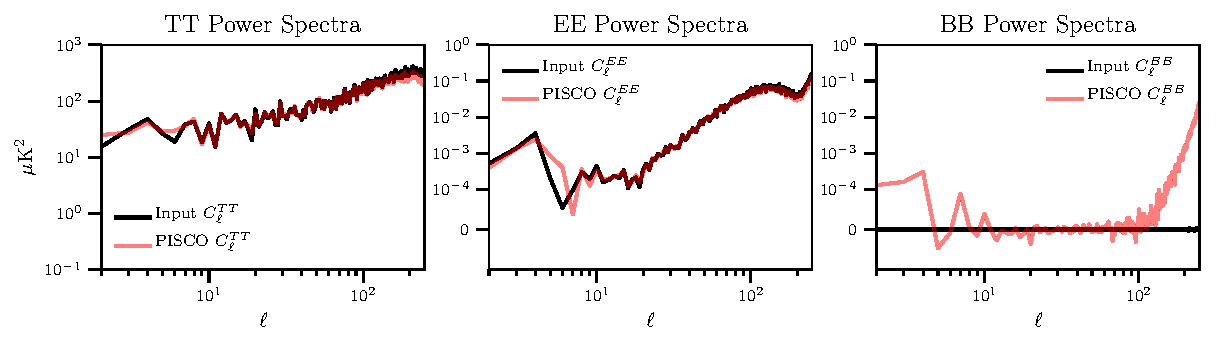
\includegraphics[width=1.0\linewidth]{figures/cmb_r0d00_CLASS_mismatchedPointing_matchedBeams_ellipticalBeams.pdf}
%	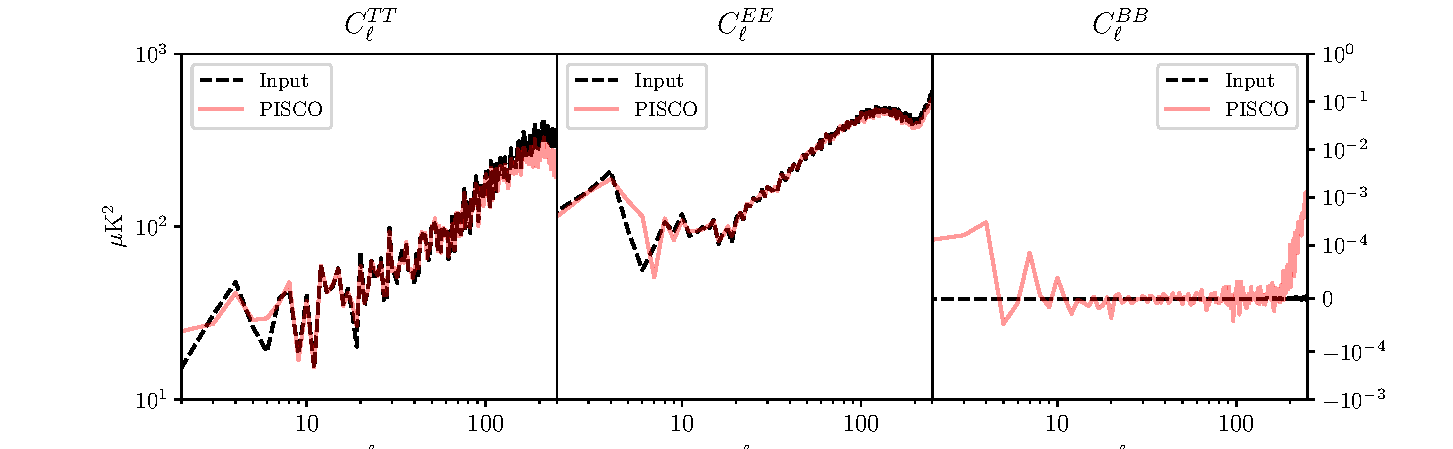
\includegraphics[width=1.0\linewidth]{figures/cmb_r0d00_CLASS_matchedPointing_matchedBeams_ellipticalBeams.pdf}
%	\caption{Upper plot. Run using an polarized CMB without B-modes as input. Focal plane has mismatched pointing for all pairs. Pointing was generated so as to emulate the CLASS scanning strategy. using this mismatch between pairs as well. Beams follow elliptical Gaussian profiles, and beam parameters are shared within pairs. Results from this experiment are in qualitative agreement with Figure \ref{fig::unpolcmbr0}, with the maximum of the spurious $BB$ spectrum reaching $\approx 50$ nK at $\ell=250$. Bottom plot: same run using matched pointing and mismatched beams. The only systematic that can explain the observed spurious $BB$ signal corresponds to asymmetric intrapixel coverage. We note that the maximum amplitude of this effect is almost two order of magnitude below  T to P leakage caused by mismatched pointing. This, together with the results of the previous section, strongly suggest this effect to origin from P to P leakage. }
%	
%	\label{fig:unpolcmbr0}
%\end{figure}

\subsubsection{Effect of beam mismatch}

Another source of leakage comes from beam mismatch. It is worth noting that this effect, if present, would dominate the signal from the power spectra at $ell$ comparable to the inverse of the beam FWHM which, for this application case, is $\approx 1.45^\circ$ corresponding to $\ell = 124$. At these scales, pointing mismatch and noise caused by uneven intra-pixel coverage also play an important role, so it becomes mandatory to suppress these systematics. The way we addressed this was to force the pointing of the scanning strategy to hit the center of pixels of an NSIDE=512 HEALPix grid. 

(PF maybe show some results from map stats here?)

Simulations were performed using this pixelated pointing stream for the case of matched and mismatched beams. 

\subsection{Discussion}

\section{Realistic CMB experiment with non zero cross-polarized beams}

\section{Conclusion}
\label{sec::conclusions}

In this work, we have presented PISCO, a new computer simulation code capable of computing tensor convolutions in pixel space for applications in CMB experiments. PISCO was also designed to use GPU acceleration, as well as supporting execution on HPC facilities. PISCO is also unique in its field, being capable of explicitly including time-dependent phenomena present in the data, like modulation techniques, beam degradation due to mechanical effects and transient events on the sky. Application of these capabilities to a realistic CMB experiment will be given in future publications.

\bibliographystyle{plain}
\bibliography{bib}

\appendix
%\numberwithin{equation}{section}	
\section{Computation of antenna coordinates from sky coordinates and antenna pointing}

In this appendix we introduce an additional coordinate system, the \textsl{instrument basis} which is a spherical coordinate system with unit base vectors $\hat{x}'$, $\hat{y}'$ and $\hat{z}'$ and spherical coordinates $\theta'$ and $\phi'$. For any given beam center pointing $\bar{q}_0$ in the sky basis, the pointing direction unit vector $\hat{p}_0$ points to the sky at the equator and prime meridian $(\theta'_0,\phi'_0) = (90,0)$ so that the unit vectors $\hat{\theta}'_0$ and $\hat{\phi}'_0$ at that point form the unit base vectors of the antenna basis coordinate system. It is natural for PISCO to adopt Ludwig's 2nd definition of cross polarization \cite{1140406} as this aligns the unit vectors $(\hat{e}_{\co},\hat{e}_{\cx})$ with $(\hat{\theta}',\hat{\phi}')$ for a detector with orientation angle $\zeta = 0$. In particular, this means that, for any beam center pointing $\bar{q}_0 = (90,\phi,0)$ in the sky basis, the co and cross polarization unit vectors are aligned with the Stokes parameters $+U$ and $-U$ respectively across the entire sky.

For a beam center pointing $\bar{q}_0$ and off beam center pointing $\bar{q}$ in the sky basis, we can derive the antenna basis coordinates $(\rho,\sigma)$, the instrument basis coordinates $(\theta',\phi')$ and the angle $\psi$ between $\hat{e}_{\co}$ and $+U$ ($\hat{\theta}$) by using spherical trigonometry (see Figure \ref{fig::figure10}). 

\begin{figure}
	\centering
	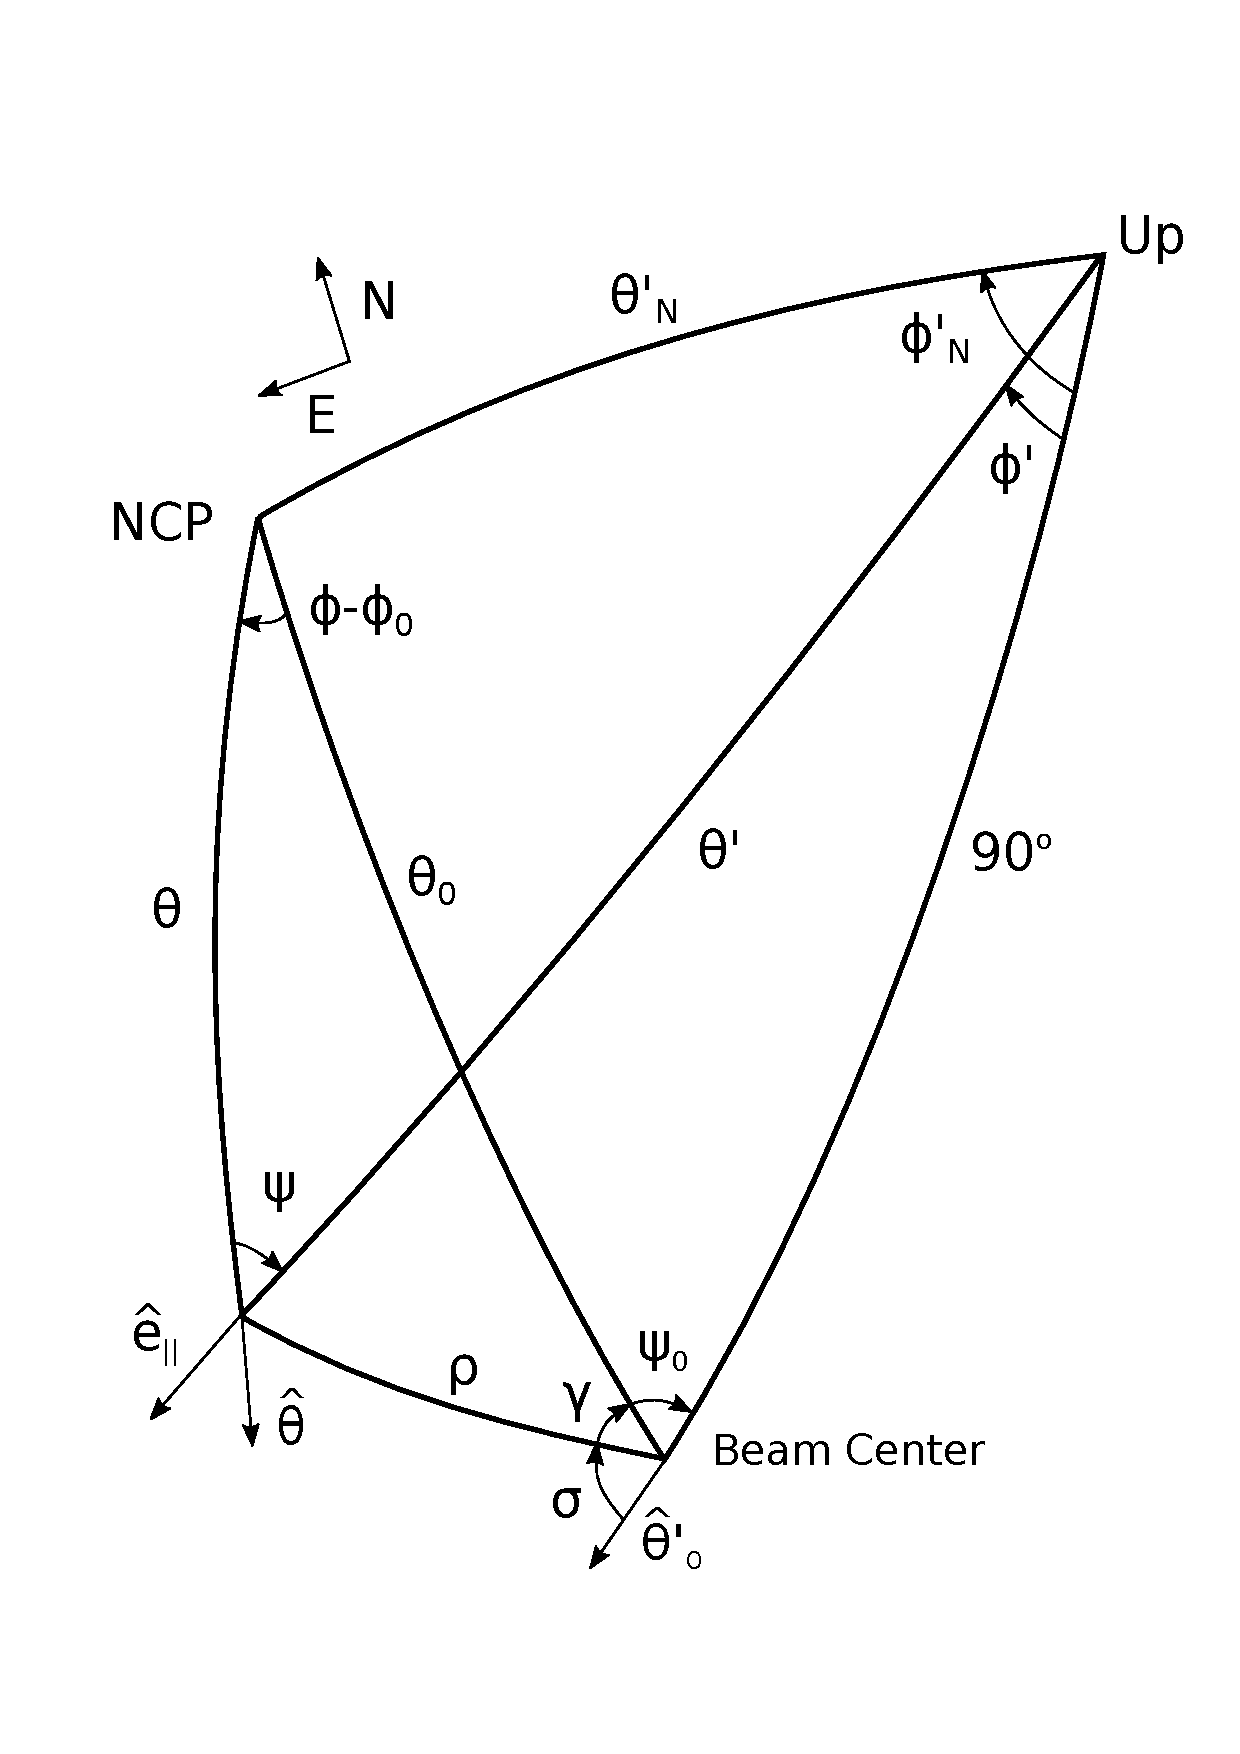
\includegraphics[width=0.8\linewidth]{figures/Figure10.pdf}
	\caption{Sky, instrument and antenna basis coordinates for beam center pointing $\bar{q_0}$ and off beam center pointing $\bar{q}$. Here $\mathrm{\texttt{NCP}}$ is the ICRS North Celestial Pole and $\mathrm{\texttt{Up}}$ is the pole in the upward direction of the instrument basis coordinate system. The instrument basis coordinates of the NCP are $(\theta'_N,\phi'_N)$.}
	\label{fig::figure10}
\end{figure}

Defining $\Delta \phi \equiv \phi - \phi_0$, the antenna basis coordinates $(\rho,\sigma)$ are given by
%
\begin{flalign}
\rho  &= \arccos( \cos(\theta) cos(\theta_0) + \sin(\theta) \sin(\theta_0) \cos(\Delta \phi) ) \nonumber & \\
\sin(\gamma) &= \frac{\sin(\theta) \sin(\Delta \phi)}{\sin(\rho)} \nonumber & \\
\cos(\gamma) &= \frac{\cos(\theta) \sin(\theta_0) - \sin(\theta) \cos(\theta_0) \cos(\Delta \phi)}{\sin(\rho)} & \\ 
\gamma       &=  \arctan \left(\frac{\sin(\theta) \sin(\Delta \phi)}{\cos(\theta) \sin(\theta_0) - \sin(\theta) \cos(\theta_0) \cos(\Delta \phi)} \right) \nonumber & \\
\sigma &= 180^{\circ} - \psi_0 - \gamma \nonumber &
\end{flalign}
%
Then the instrument basis coordinates $(\theta', \phi')$ are
%
\begin{flalign}
\theta' &= \arccos(-\sin(\rho) \cos(\sigma)) \nonumber & \\
\sin(\phi') &= \frac{\sin(\rho) \sin(\sigma)}{\sin(\theta')} \nonumber & \\
\cos(\phi') &= \frac{\cos(\rho)}{\sin(\theta')} & \\
\phi'       &= \arctan \left( \frac{\sin(\rho) \sin(\sigma)}{\cos(\rho)} \right) \nonumber &
\end{flalign}
%
For the instrument basis coordinates $(\theta'_N,\phi'_N)$, we have
%
\begin{flalign}
\theta'_N    &= \arccos(\sin(\theta_0) \cos(\psi_0)) \nonumber & \\
\sin(\phi'_N) &= \frac{\sin(\theta_0)  \sin(\psi_0)}{\sin(\theta'_N)}  & \\
\cos(\phi'_N) &= \frac{\cos(\theta_0)}{\sin(\theta'_N)} \nonumber & \\ 
\phi'_N       &= \arctan\left( \frac{\sin(\theta_0)  \sin(\psi_0)}{\cos(\theta_0)} \right) \nonumber &
\end{flalign}
%
Then, defining $\Delta \phi' \equiv \phi'_N - \phi'$, yields
%
\begin{flalign}
\cos(\psi) &= \frac{\cos(\theta'_N) \sin(\theta') - \sin(\theta'_N) \cos(\theta') \cos(\Delta \phi')}{\cos(\theta)}  \nonumber & \\
\sin(\psi) &= \frac{\sin(\theta'_N) \sin(\Delta \phi')}{\cos(\theta)}  & \\
\psi       &= \arctan\left( \frac{\sin(\theta'_N) \sin(\Delta \phi')}{\cos(\theta'_N) \sin(\theta') - \sin(\theta'_N) \cos(\theta') \cos(\Delta \phi')} \right)  \nonumber &
\end{flalign}

\section{Calculation of elements of $B$}

A beamsor $B$ evaluated at antenna basis coordinates $(\rho,\sigma)$ is a $4 \times 4$ matrix with elements

\begin{equation}
\begin{aligned}
B(\rho,\sigma) = \frac{1}{\tilde{\Omega}}
\begin{bmatrix}
B_{TT} & B_{QT} & B_{UT} & B_{VT}\\
B_{TQ} & B_{QQ} & B_{UQ} & B_{VQ}\\
B_{TU} & B_{QU} & B_{UU} & B_{VU}\\
B_{TV} & B_{QV} & B_{UV} & B_{VV}
\end{bmatrix}
\end{aligned}
\label{eq::beamsor_appendix}
\end{equation}

\noindent
with $\tilde{\Omega}$ being a normalization factor computed as

\begin{equation}
\begin{aligned}
\tilde{\Omega} = \int_{4\pi} B_{TT}(\rho,\sigma) \, \mathrm{d} \Omega
\end{aligned}
\end{equation}

The definition of a beamsor used in this work differs from the one listed in \cite{2007MNRAS.376.1767O} in that element $B_{XY}$ corresponds to element $B_{YX}$. We believe this definition yields a clearer interpretation of beamsor elements. Consider, for instance, the product of $B$ with a Stokes vector representing an unpolarized source. This yields

\begin{equation}
\begin{aligned}
\begin{bmatrix} 
B_{TT} \\ 
B_{TQ} \\ 
B_{TU} \\ 
B_{TV} 
\end{bmatrix}
=
\begin{bmatrix}
B_{TT} & B_{QT} & B_{UT} & B_{VT}\\
B_{TQ} & B_{QQ} & B_{UQ} & B_{VQ}\\
B_{TU} & B_{QU} & B_{UU} & B_{VU}\\
B_{TV} & B_{QV} & B_{UV} & B_{VV}
\end{bmatrix}
\cdot
\begin{bmatrix} 
1 \\ 
0 \\ 
0 \\ 
0 
\end{bmatrix}
\end{aligned}
\label{eq::unpol_beamsor}
\end{equation}

\noindent
where it is more evident that elements $B_{TX}$, with $X=Q,U,V$, correspond to the temperature to polarization leakage beams. 

In most CMB applications, linearly polarized detectors are placed at the focus of the antenna. In general, power that was radiated as pure $+Q$ in the detector basis will reach the sky as both $+Q$ and $-Q$ in the antenna basis. This effect can be modeled by introducing co-polar and cross-polar beams. The co-polar beam, $b_{\co}(\rho,\sigma)$, is the unit-normalized power density distribution that reaches the sky with a polarization state parallel to $\hat{e}_{\co}$. The cross-polar $b_{\cx}(\rho,\sigma)$ does so parallel to $\hat{e}_{\cx}$. 

The work of \cite{2007A&A...470..771J} also provides a way of calculating beamsor elements. Given the coordinate system convention used in this work, it is important to re-specify the way these elements are calculated. We start by considering the antenna to broadcast power originated by a linearly polarized source radiating at the location of the detection device. This will produce a distribution of electric fields in the far field, $\vec{E} = \vec{E}(\rho,\sigma)$, where $\vec{E}(\rho,\sigma)$ will have co-polarized and cross polarized components. Take $x$ to be a source oriented such that most of its radiated power reaches the sky as electric fields aligned with $\hat{\theta}'$ at beam center. Similarly, consider another source, $y$, aligned perpendicularly such that most its transmitted power reaches the sky as electric fields aligned with $\hat{\phi}'$, at beam center. In this situation, elements of a beamsor can be computed via

\begin{equation}
\begin{split}
B_{TT}&=\frac{1}{2}\left(\left|\vec{E}_{x}\right|^{2}+\left|\vec{E}_{y}\right|^{2}\right)\\
B_{QT}&=\frac{1}{2}\left(\left|\vec{E}_{x,\co}\right|^{2}-\left|\vec{E}_{x,\cx}\right|^{2} +  \left|E_{y,\cx}\right|^{2}-\left|E_{y,\co}\right|^{2}\right)\\
B_{UT}&=\frac{1}{2}\left(\vec{E}_{x,\co} E_{x,\cx}^{*} - E_{y,\co} E_{y,\cx}^{*}\right) + \mathrm{c.c.}\\
B_{VT}&=\frac{1}{2}\mathrm{i}\left(\vec{E}_{x,\co}\vec{E}_{x,\cx}^{*} + \vec{E}_{y,\co} \vec{E}_{y,\cx}^{*}\right) + \mathrm{c.c.}\\
B_{TQ}&=\frac{1}{2}\left(\left|\vec{E}_{A}\right|^{2}-\left|\vec{E}_{B}\right|^{2}\right)\\
B_{QQ}&=\frac{1}{2}\left(\left|\vec{E}_{x,\co}\right|^{2}-\left|\vec{E}_{x,\cx}\right|^{2}+\left|\vec{E}_{y,\co}\right|^{2}-\left|\vec{E}_{y,\cx}\right|^{2}\right)\\
B_{UQ}&=\frac{1}{2}\left(\vec{E}_{x,\co} \vec{E}_{x,\cx}^{*} + \vec{E}_{y,\co} \vec{E}_{y,\cx}^{*}\right)+\mathrm{c.c.}\\
B_{VQ}&=\frac{1}{2}\mathrm{i}\left( \vec{E}_{x,\co} E_{x,\cx}^{*} - E_{y,\co} E_{y,\cx}^{*}\right)+\mathrm{c.c.}\\
B_{TU}&=\frac{1}{2}\left( -\vec{E}_{x,\co} \vec{E}_{x,\cx}^{*} + \vec{E}_{y,\cx} \vec{E}_{y,\co}^{*}\right)+\mathrm{c.c.}\\
B_{QU}&=\frac{1}{2}\left(-\vec{E}_{x,\co}\vec{E}_{y,\cx}^{*} - \vec{E}_{x,\cx} \vec{E}_{y,\co}^{*}\right)+\mathrm{c.c.}\\
B_{UU}&=\frac{1}{2}\left(\vec{E}_{x,\co} \vec{E}_{y,\co}^{*} - \vec{E}_{x,\cx} \vec{E}_{y,\cx}^{*}\right)+\mathrm{c.c.}\\
B_{VU}&=\frac{1}{2}\mathrm{i}\left(\vec{E}_{x,\co} \vec{E}_{y,\co}^{*} + \vec{E}_{x,\cx}\vec{E}_{y,\cx}^{*}\right)+\mathrm{c.c.}\\
B_{TV}&=\frac{1}{2}\mathrm{i}\left(\vec{E}_{x,\co} \vec{E}_{y,\cx}^{*} - \vec{E}_{x,\cx}\vec{E}_{y,\co}^{*}\right)+\mathrm{c.c.}\\
B_{QV}&=\frac{1}{2}\mathrm{i}\left(\vec{E}_{\mathrm{x,\co}} \vec{E}_{y,\cx}^{*} + \vec{E}_{x,\cx} \vec{E}_{y,\co}^{*}\right)+\mathrm{c.c.}\\
B_{UV}&=\frac{1}{2}\mathrm{i}\left(-\vec{E}_{x,\co} \vec{E}_{y,\co}^{*} + \vec{E}_{A,\cx} \vec{E}_{y,\cx}^{*}\right)+\mathrm{c.c.}\\
B_{VV}&=\frac{1}{2}\left(\vec{E}_{x,\co} \vec{E}_{y,\co}^{*} + \vec{E}_{x,\cx} \vec{E}_{y,\cx}^{*}\right)+\mathrm{c.c.}
\end{split}
\end{equation}
%
\noindent
where c.c. stands for complex conjugate.

\end{document}
